%% CC-UENF-projeto-pesquisa.tex
%% Prof. Ausberto Castro Vera
%% URNF - CCT - LCMAT - CC
%% 2016-2021
%%  Informa\c{c}\~{o}es do Projeto de TCC

% verso e anverso:
%\documentclass[12pt,openright, twoside,a4paper,english,brazil]{abntex2}	

% apenas verso:
\documentclass[12pt,oneside,a4paper,english,brazil]{abntex2}	

\usepackage{titlesec}

\titleformat{\chapter}[display]
{\normalfont\huge\bfseries}{Capítulo \thechapter : }{0cm}{\Huge}

% ---
% Pacotes fundamentais 
% ---
%\usepackage{sbc-template}
\usepackage{cmap}				% Mapear caracteres especiais no PDF
\usepackage{lmodern}			% Usa a fonte Latin Modern
\usepackage[T1]{fontenc}		% Selecao de codigos de fonte.
\usepackage[utf8]{inputenc}		% Codificacao do documento (convers\~{a}o autom\'{a}tica dos acentos)
\usepackage{indentfirst}		% Indenta o primeiro par\'{a}grafo de cada se\c{c}\~{a}o.
\usepackage{xcolor}				% Controle das cores
\usepackage{here}               % Fixar as imagens dentro do texto
\usepackage[table,xcdraw]{xcolor}
\usepackage{colortbl} 
\usepackage[table,xcdraw]{xcolor}

\usepackage{url}
\usepackage{quoting}
\setlength\tabcolsep{0.3cm}
\renewcommand{\arraystretch}{1.7} 


% Definindo novas cores
\definecolor{verde}{rgb}{0.25,0.5,0.35}
\definecolor{jpurple}{rgb}{0.5,0,0.35}
\definecolor{darkgreen}{rgb}{0.0, 0.2, 0.13}
\definecolor{oldmauve}{rgb}{0.4, 0.19, 0.28}

% Configurando layout para mostrar codigos Java
\usepackage{listings}

\renewcommand{\lstlistingname}{Código}
\renewcommand{\lstlistlistingname}{Lista de Códigos}

\newcommand{\estiloJava}{
\lstset{
    language=Java,
    basicstyle=\ttfamily\small,
    keywordstyle=\color{jpurple}\bfseries,
    stringstyle=\color{red},
    commentstyle=\color{verde},
    morecomment=[s][\color{blue}]{/**}{*/},
    extendedchars=true,
    showspaces=false,
    showstringspaces=false,
    numbers=left,
    numberstyle=\tiny,
    breaklines=true,
    backgroundcolor=\color{cyan!10},
    breakautoindent=true,
    xleftmargin=0pt,
    tabsize=2,
}}



\usepackage{graphicx}			% Inclus\~{a}o de gr\'{a}ficos
 \graphicspath{{Pictures/}{Imagens/}{Figuras/}} % Especifica a pasta onde  est\~{a}o armazenados os arquivos imagens
% ---

% ---
% Pacotes adicionais, usados apenas no \^{a}mbito do Modelo Can\^{o}nico do abnteX2
% ---
% Pacotes de cita\c{c}\~{o}es
% ---
\usepackage[brazilian,hyperpageref]{backref}	 % Paginas com as cita\c{c}\~{o}es na bibl
\usepackage[alf]{abntex2cite}	% Cita\c{c}\~{o}es padr\~{a}o ABNT

% ---
% CONFIGURA\c{C}\~{O}ES DE PACOTES
% ---

% ---
% Configura\c{c}\~{o}es do pacote backref
% Usado sem a op\c{c}\~{a}o hyperpageref de backref
\renewcommand{\backrefpagesname}{Citado na(s) p\'{a}gina(s):~}
% Texto padr\~{a}o antes do n\'{u}mero das p\'{a}ginas
\renewcommand{\backref}{}
% Define os textos da cita\c{c}\~{a}o
\renewcommand*{\backrefalt}[4]{
	\ifcase #1 %
		Nenhuma cita\c{c}\~{a}o no texto.%
	\or
		Citado na p\'{a}gina #2.%
	\else
		Citado #1 vezes nas p\'{a}ginas #2.%
	\fi}%
% ---


% ---
% Informa\c{c}\~{o}es de dados para CAPA e FOLHA DE ROSTO
% ---
\titulo{Um modelo de requisitos de segurança para aplicações bancárias no Android
}
\autor{José Lucio C. Azevedo }
\local{Campos dos Goytacazes, RJ}
\data{\today}                    %% <======================== MUDAR: dd Maio de 202xxxs
\orientador{Prof. Dr. Ausberto S. Castro Vera}   %% <======================== MUDAR
\coorientador{Prof. Dr. João Luiz de Almeida Filho}
\instituicao{%
  Universidade Estadual do Norte Fluminense Darcy Ribeyro
  \par
  CCT - Laborat\'{o}rio de Ciencias Matem\'{a}ticas
  \par
  Curso de Ci\^{e}ncia da Computa\c{c}\~{a}o}
\tipotrabalho{Projeto de Pesquisa (TCC)}
% O preambulo deve conter o tipo do trabalho, o objetivo,
% o nome da institui\c{c}\~{a}o e a \'{a}rea de concentra\c{c}\~{a}o
\preambulo{Projeto de pesquisa apresentado como requisito para aprovar a disciplina de Projeto de Monografia do Curso de Bacharel em Ci\^{e}ncia da Computa\c{c}\~{a}o, da Universidade Estadual do Norte Fluminense Darcy Ribeiro}
% ---

% ---
% Configura\c{c}\~{o}es de apar\^{e}ncia do PDF final

% alterando o aspecto da cor azul
\definecolor{blue}{RGB}{41,5,195}

% informa\c{c}\~{o}es do PDF
\makeatletter
\hypersetup{
     	%pagebackref=true,
		pdftitle={\@title},
		pdfauthor={\@author},
    	pdfsubject={\imprimirpreambulo},
	    pdfcreator={\@author, LaTeX with abnTeX2},
		pdfkeywords={abnt}{latex}{abntex}{abntex2}{projeto de pesquisa},
		colorlinks=true,       		% false: boxed links; true: colored links
    	linkcolor=red,          	% color of internal links
    	citecolor=blue,        		% color of links to bibliography
    	filecolor=magenta,      		% color of file links
		urlcolor=blue,
		bookmarksdepth=4
}
\makeatother
% ---

% ---
% Espa\c{c}amentos entre linhas e par\'{a}grafos
% ---

% O tamanho do par\'{a}grafo \'{e} dado por:
\setlength{\parindent}{1.3cm}

% Controle do espa\c{c}amento entre um par\'{a}grafo e outro:
\setlength{\parskip}{0.2cm}  % tente tamb\'{e}m \onelineskip

% ---
% compila o indice
% ---
\makeindex
% ---

% ----
% In\'{\i}cio do documento
% ----
\begin{document}

% Retira espa\c{c}o extra obsoleto entre as frases.
\frenchspacing

% ----------------------------------------------------------
% ELEMENTOS PR\'{E}-TEXTUAIS
% ----------------------------------------------------------
% -------------------------------------------------
% Prof. Dr. Ausberto S. Castro Vera
% UENF - CCT - LCMAT - Curso de Ci\^{e}ncia da Computa\c{c}\~{a}o - Matem\'{a}tica - PROFMAT
% Campos, RJ,  2013-2022
% Curso de LaTeX
% -------------------------------------------------
%%  Informa\c{c}\~{o}es do Projeto de TCC
% -------------------------------------------------


% ----------------------------------------------------------
% ELEMENTOS PR\'{E}-TEXTUAIS
% ----------------------------------------------------------
% \pretextual 

% ---
% Capa
% ---
\imprimircapa
% ---

% ---
% F olha de rosto
% ---
\imprimirfolhaderosto
% ---

% ---
% NOTA DA ABNT NBR 15287:2011, p. 4:
%  ``Se exigido pela entidade, apresentar os dados curriculares do autor em
%     folha ou p\'{a}gina distinta ap\'{o}s a folha de rosto.''
% ---

\begin{folhadeaprovacao}


\begin{center}
    {\ABNTEXchapterfont\large\imprimirautor}

    \vspace*{\fill}\vspace*{\fill}
    \begin{center}
      \ABNTEXchapterfont\bfseries\Large\imprimirtitulo
    \end{center}
    \vspace*{\fill}

\end{center}

Projeto de pesquisa apresentado como requisito da disciplina de Projeto de Monografia do Curso de Bacharel em Ciência da Computação, da Universidade Estadual do Norte Fluminense Darcy Ribeiro, sendo aprovada em sua forma final pela banca examinadora:

    \vspace{1.5cm}
    \assinatura{\textbf{Prof. Dr. Ausberto S. Castro Vera} \\ Orientador}
    \assinatura{\textbf{Prof. Dr. João Luiz de Almeida Filho} \\ Coorientador}
    \assinatura{\textbf{Prof. Dr. Fermín Alfredo Tang Montané} \\ Membro da banca}
    \assinatura{\textbf{Prof. Dr. Luis Alberto R. Ramirez}\\ Membro da banca}
    \vspace{3 cm}%\vfill

    \begin{center}
    \vspace*{0.5cm}
    {\large\imprimirlocal}
    \par
    {\large28 de agosto de 2024}
    \vspace*{1cm}
  \end{center}
  
\end{folhadeaprovacao}

% ---
% Agradecimentos
% ---

\begin{agradecimentos}
Gostaria de expressar minha mais profunda gratidão aos meus pais e família, que desde os primeiros passos na minha vida plantaram em mim o valor da educação e da perseverança. Cada conselho, cada palavra de encorajamento e cada gesto de apoio foram fundamentais para que eu pudesse chegar até aqui.

Agradeço ao me orientador,  Prof. Dr. Ausberto S. Castro Vera, que me acompanha de perto desde o primeiro ano da minha graduação durante um projeto de iniciação científica. Sua orientação constante, paciência e ter sido uma fonte inesgotável de conhecimento e apoio ao longo desta jornada foram parte indispensável para a formação desse trabalho e de toda a minha vida acadêmica e profissional.  

Ao meu coorientador, Prof. Dr. João Luiz de Almeida Filho, agradeço imensamente por sua dedicação em me ajudar a desenvolver este projeto. Sua habilidade em traçar os caminhos e direcionar cada etapa foi essencial para que eu pudesse alcançar os objetivos propostos.

À Giovana Assis França, sou grato por ter me ajudado a idealizar este projeto desde o início. Sua visão e sugestões de uma especialista foram fundamentais para moldar o trabalho que apresento hoje.

Agradeço à minha namorada, Mariana, por todo o apoio emocional, carinho e episódio de One Piece. Cada palavra de incentivo, cada abraço reconfortante, e cada sorriso compartilhado fazem parte desse trabalho. 

Aos meus amigos, que compartilharam tantos momentos ao longo desses anos, em especial Daniel e João, meus irmãos "Sabudos - Ex IC". Vocês foram mais do que colegas, foram verdadeiros irmãos, sempre prontos para compartilhar conhecimentos sobre organização, trocar ideias filosóficas e vazias, e acima de tudo, proporcionar motivações para realizar esse grande trabalho de Sísifo chamado Monografia.


\end{agradecimentos}
% ---

\begin{epigrafe}
  \vspace*{\fill}
  \begin{flushright}
    \textit{``Quando vocês acham que as pessoas morrem? \\
            Quando elas levam um tiro de pistola bem no coração? Não. \\
            Quando são vencidas por uma doença incurável? Não! \\
            Quando bebem uma sopa de cogumelo venenoso? Não! \\
            Elas morrem... Quando são esquecidas.''\\
      Dr. Hiluluk}
  \end{flushright}
\end{epigrafe}

% resumo em português
\setlength{\absparsep}{18pt} % ajusta o espaçamento dos parágrafos do resumo


\begin{resumo}
Esta monografia apresenta um estudo detalhado sobre a segurança em aplicações bancárias no sistema operacional Android, com o objetivo de desenvolver um modelo de requisitos de segurança específico para essas aplicações. Dada a crescente popularidade dos dispositivos móveis e a frequência com que são utilizados para realizar transações financeiras, garantir a segurança dessas operações tornou-se uma prioridade crucial. O trabalho realiza uma análise abrangente das vulnerabilidades e ameaças associadas aos aplicativos bancários no sistema operacional Android, além de explorar os métodos de mitigação mais eficazes para esses problemas. Para identificar e entender os pontos críticos de segurança, foi feita uma revisão na literatura e utilizada a ferramenta de análise de casos de uso indevido, permitindo uma compreensão profunda das possíveis falhas e riscos. A partir dessa análise, é proposto um modelo detalhado de requisitos de segurança, específico para o contexto das aplicações bancárias no Android, e estruturado através de diagramas UML. Este modelo inclui diretrizes claras e práticas para garantir a confidencialidade, integridade, autenticação e autorização dos dados. Finalmente, o modelo é avaliado por meio de um estudo de caso aplicado à Herd Financial e de uma avaliação de conformidade utilizando a certificação PCI DSS, demonstrando como os requisitos de segurança propostos podem ser implementados e como eles garantem a segurança da aplicação. Esta monografia modela uma solução prática e implementável para garantir a proteção dos dados dos usuários e a confiança nos serviços bancários móveis; assim, destacando a importância de medidas de segurança robustas e oferece uma contribuição significativa aos desenvolvedores e provedores desse serviço.

 \textbf{Palavras-chave}: Segurança da informação. Aplicações bancárias móveis. Android. Engenharia de requisitos.
\end{resumo}

% resumo em inglês
\begin{resumo}[Abstract]
 \begin{otherlanguage*}{english}
This monograph presents a detailed study on the security of banking applications on the Android operating system, with the goal of developing a specific set of security requirements for these applications. Given the growing popularity of mobile devices and their frequent use for financial transactions, ensuring the security of these operations has become a critical priority. The work provides a comprehensive analysis of the vulnerabilities and threats associated with banking applications on the Android operating system, as well as exploring the most effective mitigation methods for these issues. To identify and understand the critical security points, a literature review was conducted, and the misuse case analysis tool was used, allowing a deep understanding of potential failures and risks. Based on this analysis, a detailed security requirements model is proposed, specifically tailored to the context of banking applications on Android, structured through UML diagrams. This model includes clear and practical guidelines to ensure data confidentiality, integrity, authentication, and authorization. Finally, the model is evaluated through a case study applied to Herd Financial and an assessment of compliance with the PCI DSS certification, demonstrating how the proposed security requirements can be implemented and how they ensure the application's security. This thesis models a practical and implementable solution to ensure the protection of user data and trust in mobile banking services, highlighting the importance of robust security measures and offering a significant contribution to developers and providers of this service.
   \vspace{\onelineskip}
 
   \noindent 
   \textbf{Keywords}: Information security. Mobile Banking. Android. Requirements engineering.
 \end{otherlanguage*}
\end{resumo}


% ---
% inserir lista de ilustra\c{c}\~{o}es
% ---
\pdfbookmark[0]{\listfigurename}{lof}
\listoffigures*
\cleardoublepage
% ---

% ---
% inserir lista de tabelas
% ---
\pdfbookmark[0]{\listtablename}{lot}
\listoftables*
\cleardoublepage
% ---

\pdfbookmark[0]{\listfigurename}{lof}

\begin{siglas}

\item[FEBRABAN] Federação Brasileira de Bancos
\item[API] Application Programming Interface
\item[GUI] Graphical User Interface
\item[SD Card] Secure Digital Card
\item[IPC] Inter-Process Communication
\item[OWASP] Open Web Application Security Project
\item[SSL] Secure Sockets Layer
\item[TLS] Transport Layer Security
\item[DDoS] Distributed Denial of Service
\item[DoS] Denial of Service
\item[IPS] Intrusion Prevention System
\item[XSS] Cross-site scripting
\item[URL] Uniform Resource Locator
\item[OTP] One-Time Password
\item[TOTP] Time-based One-Time Password
\item[PIN] Personal Identification Number
\item[MFA] Multi-Factor Authentication
\item[PCI DSS] Payment Card Industry Data Security Standard
\item[MASVS] Mobile Application Security Verification Standard
\item[UML] Unified Modeling Language
\item[Crypto] Cryptography 
\item[AES-256-CBC] Advanced Encryption Standard com uma chave de 256 bits no modo Cipher Block Chaining
\item[SHA-256] Secure Hash Algorithm com valor hash de 256 bits
\item[ECDSA] Elliptic Curve Digital Signature Algorithm 


\end{siglas}
\cleardoublepage

% ---
% inserir o sumario
% ---
\pdfbookmark[0]{\contentsname}{toc}
\tableofcontents*
\cleardoublepage
% ---



% ----------------------------------------------------------
% ELEMENTOS TEXTUAIS
% ----------------------------------------------------------
\textual

% ----------------------------------------------------------
% Introdu\c{c}\~{a}o
% ----------------------------------------------------------


    \chapter{Introdução}

    Desde os tempos antigos os m\'{e}todos de pagamento e manipulação de dinheiro vêm mudando de maneira constante. Segundo \citeonline{tellez2017}, antes de haver um sistema monetário o pagamento era feito com trocas de mercadoria e isso foi eficiente enquanto as necessidades humanas eram limitadas. Entretanto, com o crescimento da complexidade da sociedade, este método se tornou insuficiente e o homem teve que adotar outros sistemas como moedas de minério, e após isso, dinheiro e o cart\~{a}o banc\'{a}rio. Com o avanço tecnológico, rápido desenvolvimento da tecnologia de redes móveis e os avanços nos dispositivos portáteis, tornou-se possível que as pessoas acessassem a Internet usando dispositivos móveis em qualquer lugar e a qualquer hora para realizar transações de comércio eletrônico e outras operações, como navegação na web, leitura de e-mail e assim por diante. Dessa forma, foi possível a criação de novos m\'{e}todos pr\'{a}ticos, fáceis e r\'{a}pidos de pagamento e manipulação de dinheiro.
    
    
    O banco móvel, segundo \citeonline{Singhal2019}, se refere à provisão de serviços bancários, tais como transferências, verificação de saldos, efetuação de pagamentos, investimentos e outras transações, através de dispositivos portáteis que suportam aplicativos - smartphones, tablets e, em alguns casos, smartwatches. Com essa capacidade, os clientes têm à disposição a maioria dos serviços oferecidos por suas instituições financeiras na palma de suas mãos, sem a necessidade de visitar uma agência bancária ou um caixa eletrônico, nem de estar em frente a um computador de mesa ou laptop. 
    
    As estatísticas \cite{Deloitte2021} confirmam que a adoção dessa abordagem de interação com as instituições financeiras está ganhando força. Na figura \ref{MobileBanking} pode-se observar alguns exemplos de bancos que fornecem aplicações bancárias, como Banco do Brasil, Bradesco, Caixa, Itaú e Santander.

    \begin{figure}[H]
    \centering 
    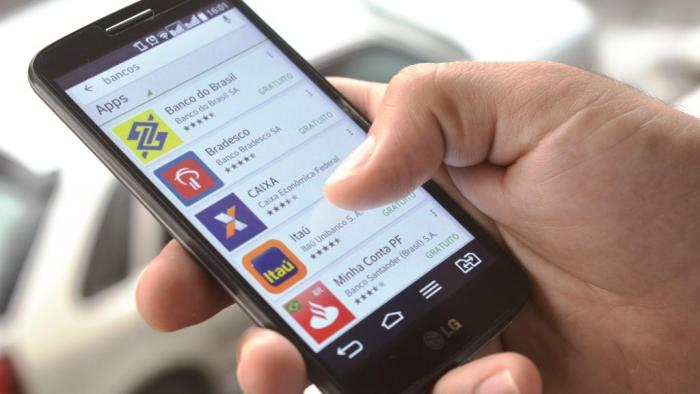
\includegraphics[width = 10cm]{Imagens/mobilebanking.jpg}
    \caption{Aplicações de banco móvel}
    \label{MobileBanking}
    \end{figure}
    
    Uma pesquisa encomendada pela Federação Brasileira de Bancos (FEBRABAN) e realizada pela empresa \citeonline{Deloitte2021} sobre tecnologia bancária revelou um aumento de 20\% no número de transações realizadas por dispositivos móveis de 2019 para 2020. Enquanto em 2019 foram efetuadas 37 bilhões de transações, no ano seguinte esse número saltou para 52,9 bilhões. Esse crescimento foi impulsionado pela pandemia e pelo programa de auxílio emergencial e essa combinação de fatores consolidou os celulares e outros dispositivos móveis como um dos principais canais de atendimento no setor bancário, como apresentado na figura \ref{febran}.
    
    \begin{figure}[H]
    \centering 
    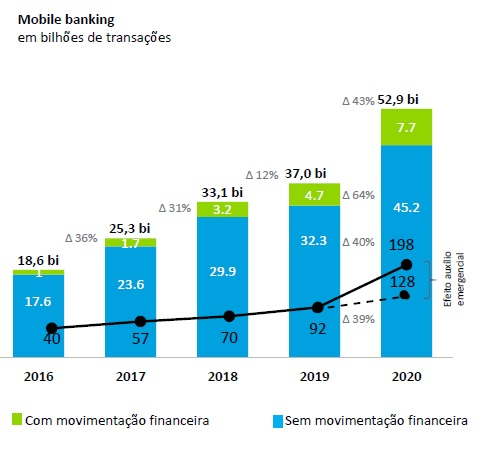
\includegraphics[width = 11cm]{Imagens/febran.jpg}
    \caption{Número de transações mobile}
    Fonte: \citeonline{Deloitte2021}
    \label{febran}
    \end{figure}
    
    
    Nesse sentido, a segurança da informação desempenha um papel fundamental no contexto das aplicações bancárias móveis. Dada a crescente popularidade destas tecnologias, é importante garantir que os dados sensíveis dos utilizadores sejam protegidos. As transações financeiras e o acesso a informações pessoais estão em risco, e as violações de segurança podem ter consequências graves, como furto financeiro, fraude e até mesmo comprometimento da identidade do usuário. Dessa forma, investir em medidas de segurança robustas não apenas tranquilizará seus clientes, mas também aumentará sua confiança ao usar esses aplicativos. 
    
    A segurança da informação não é apenas uma prioridade, mas uma necessidade para que os serviços bancários móveis continuem a evoluir e a beneficiar os consumidores de uma forma segura e eficaz. Para fazer esses aplicativos seguros é importante entender os problemas de segurança que ele traz, como por exemplo dispositivos perdidos, riscos na rede, senhas fracas, vazamentos e erros humanos. Muitas vezes, a implementação indevida ou a falta da segurança nas aplicações financeiras abre brechas para invasores. Como esse tipo de aplicativo lida diretamente com o dinheiro, eles mais do que qualquer outro devem ter a segurança impecável e lidar com esses problemas citados.
    
    Em 2015, dois pesquisadores, \citeonline{DIEGO2015}, da Universidade Estadual de Campinas (Unicamp) realizaram um estudo para identificar deficiências e fragilidades nos aplicativos de alguns bancos gigantes brasileiros para android e o resultado foi no mínimo problemático. Como mostrado na Figura \ref{PesquisaUnicamp}, foi descoberto que alguns desses aplicativos utilizavam métodos extremamente básicos de segurança e muitas vezes sabidamente vulneráveis a ataques de segurança simples, como ataques de interceptação de dados e vazamento de dados. Foram dadas notas que variam de 0 a 5 estrelas para as aplicações do topo da tabela com base na vulnerabilidade aos ataques listados na esquerda da tabela, sendo o número de estrelas diretamente proporcional qualidade da segurança da aplicação. Dessa forma, a aplicação com mais estrelas é a menos vulnerável aos ataques e a com menos estrelas é a mais vulnerável.   
    
    \begin{figure}[H]
    \centering 
    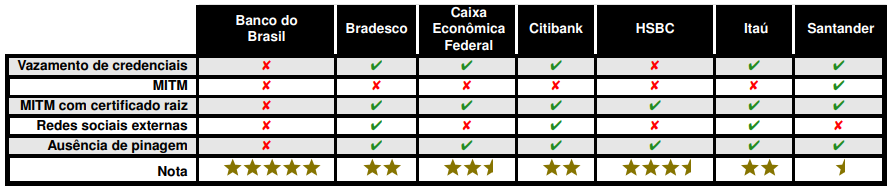
\includegraphics[width = 15cm]{Imagens/pesqunicamp.png}
    \caption{Resultado dos aplicativos Android analisados}
    \label{PesquisaUnicamp}
    Fonte: \citeonline{DIEGO2015}
    \end{figure}

    Somado a isso, como dito por \citeonline{Wang2016}, os ataques de hackers a aplicações e serviços bancários são uma ameaça crescente e significativa no mundo digital. À medida que o uso dessas tecnologias aumenta, os cibercriminosos exploram vulnerabilidades para obter acesso às informações financeiras confidenciais dos usuários e estão constantemente desenvolvendo estratégias avançadas.
    
    A todo instante são estudadas formas de desenvolver aplicações cada vez mais seguras e blindadas de ataques, identificar vulnerabilidade e propor correções antes de serem encontradas por algum indivíduo de fato malicioso. Entretanto, as aplicações bancárias incorporam características específicas, descritas por \citeonline{Islam2014}, e para garantir a segurança da informação em um cenário digital é cada vez mais complexo. 
         
    
    \section{Problemática}
    As aplicações bancárias são alvos atraentes para cibercriminosos devido à quantidade significativa de informações sensíveis que manipulam, incluindo dados pessoais, credenciais de acesso e informações financeiras. A complexidade do ecossistema móvel, combinada com práticas inadequadas de desenvolvimento e a crescente sofisticação dos ataques cibernéticos, aumenta a probabilidade de vulnerabilidades exploráveis. Tais vulnerabilidades podem resultar em ataques e outras formas de exploração que comprometem a segurança dos usuários e das instituições financeiras.
    
    A diversidade das áreas, métodos e práticas de segurança tornam difícil estabelecer diretrizes comuns e mais críticas levando em consideração as características específicas das aplicações financeiras, criando uma lacuna potencial na proteção dos dados e recursos dos usuários. 
    
    \section{Hipótese}
    A proposta de um modelo de requisitos de segurança, com base em uma revisão da literatura ressaltando ameaças e remediações eficazes, pode estabelecer diretrizes claras para o desenvolvimento seguro dessas aplicações no Android, abordando aspectos e cenários específicos do meio financeiro digital.
    
    \section{Objetivos} 
    
    O objetivo geral deste presente trabalho é propor um modelo de segurança para plataformas bancárias no Android, que seja capaz de mitigar os principais riscos e ameaças encontrados no cenário, bem como contribuir para a compreensão aprofundada e promoção da segurança da informação nessas aplicações. 
    
    Os objetivos específicos incluem:

    \begin{itemize}[topsep=3pt, partopsep=3pt, itemsep=3pt, parsep=3pt]
        \item Pesquisa: Realizar uma pesquisa de revisão visando entender, selecionar e desmistificar os principais pontos críticos de segurança em aplicações bancárias móveis e suas remediações.
        \item Criação: Propor um modelo de requisitos de segurança, com base nas informações obtidas na pesquisa anterior, que mitigue as principais ameaças encontradas.  
        \item Avaliação: Avaliar a eficácia e a viabilidade do modelo de requisitos de segurança proposto por meio de uma análise comparativa com certificações de segurança reconhecidas no mercado e de um estudo de caso. 
    \end{itemize}
    
    \section{Justificativa} 
    
    A disseminação de aplicativos bancários móveis na plataforma Android revolucionou a maneira pela qual os indivíduos conduzem transações financeiras, oferecendo maior conveniência e acessibilidade. No entanto, esse aumento na popularidade atraiu o interesse de agentes mal-intencionados, que veem essas plataformas como alvos lucrativos para possíveis ataques cibernéticos.

    A justificativa para este trabalho reside na necessidade premente de combater essas vulnerabilidades. A segurança nos aplicativos bancários é fundamental não apenas para proteger as informações confidenciais do usuário, mas também para manter a integridade e a confiabilidade da infraestrutura financeira digital. Dada a crescente dependência das tecnologias móveis, as violações de segurança têm o potencial de levar a perdas financeiras significativas e manchar a reputação das instituições envolvidas.
    
    \section{Resultados esperados} 
    Com a conclusão deste trabalho, espera-se obter um modelo de segurança para desenvolvedores de aplicações bancárias e com isso a minimização de riscos e ameaças na implementação e uso de aplicações bancárias, promovendo uma cultura de segurança mais sólida e específica.

    \section{Organização do trabalho}
    Este trabalho foi estruturado em seis capítulos, sendo eles:  
    
    No capítulo 2, "Referencial Teórico", são abordados os principais conceitos e teorias relacionados à segurança da informação, ao sistema operacional Android, às vulnerabilidades e ameaças em aplicações bancárias móveis, e à engenharia de requisitos. Este capítulo discute os conteúdos relevantes para o desenvolvimento do modelo proposto, como a revisão da literatura a fim de buscar as maiores ameaças das aplicações bancárias. 
    
    No capítulo 3, "Metodologia da Pesquisa", descreve as metodologias utilizadas para a realização da pesquisa, incluindo o levantamento e análise de dados, a elicitação e definição de requisitos de segurança utilizando casos de uso indevido, a especificação e modelagem dos requisitos com o uso de diagramas UML, e por fim são apresentados um estudo de caso e uma avaliação do modelo de segurança proposto.
    
    No capítulo 4, "Análise de Requisitos de Segurança", são detalhados os processos de elicitação, definição e especificação dos requisitos de segurança identificados, com base nos casos de uso indevido e a modelagem dos requisitos, através de diagramas UML, ilustrando a estrutura e interações dos componentes do sistema.
    
    O capítulo 5, "Estudo de caso e Avaliação do Modelo", aborda um estudo de caso do modelo de segurança proposto em um ambiente de teste, com uma análise detalhada dos casos de uso do modelo na aplicação bancária Herd Financial. Além disso, eficácia do modelo é avaliada por meio de comparações com padrões de segurança exigidos e reconhecidos no mercado.
    
    Finalmente o capítulo 6, "Conclusão",apresenta as conclusões do estudo, destacando as contribuições do trabalho, as limitações encontradas e sugestões para pesquisas futuras.



    \chapter{Referencial teórico}
    
    \section{Segurança da informação}
    Segurança da informação é o conjunto de práticas, políticas, procedimentos e tecnologias que tem como objetivo proteger as informações de uma organização. A segurança de uma determinada informação pode ser afetada por fatores comportamentais e de uso de quem se utiliza dela, pelo ambiente ou infraestrutura que a cerca ou por pessoas mal intencionadas que têm o objetivo de furtar, destruir ou modificar tal informação.
    
    Para implementar aplicações seguras, \citeonline{Hintzbergen2018} descreve que é necessário implementar um conjunto adequado de controles, políticas, processos, procedimentos, estruturas e funções tanto de software, quanto de hardware. Existe a necessidade de estabelecer, implementar, monitorar, revisar e melhorar onde necessário, para ter certeza que os objetivos específicos da segurança da informação estão sendo atendidos. Esse objetivo é manter os pilares principais da segurança da informação, que são a confidencialidade, integridade, disponibilidade e, mesmo não citados em todas as literaturas, autenticidade e não-repúdio.
    
    \subsection{Confidencialidade}
    A confidencialidade, segundo \citeonline{Machado2014}, se refere a capacidade de garantir que o nível necessário de sigilo seja aplicado em cada junção de dados em processamento. Além disso, trata-se dos limites em termos de quem pode obter que tipo de informação, isso é, o ato de garantir que a informação seja acessível apenas àqueles autorizados a ter acesso. Nomes, CPFs, números de cartão, transações e registros financeiros, entre outras informações sensíveis, devem ter acesso autorizado somente aos indivíduos com permissão para ver tal informação. 
    
    Ela garante que o nível necessário de sigilo seja aplicado em cada elemento de processamento de dados e impede a divulgação não autorizada. Esse nível de confidencialidade deve prevalecer enquanto os dados residirem em sistemas e dispositivos na rede, quando forem transmitidos e quando chegarem ao seu destino.
    
    Este pilar pode ser fornecida através da criptografia de dados à medida que são armazenados e transmitidos, usando preenchimento de tráfego na rede, estrito controle de acesso, classificação dos dados e treinamento de pessoal nos procedimentos apropriados.
    
    \subsection{Integridade}
    A integridade, segundo \citeonline{Machado2014}, é a garantia de rigor e confiabilidade das informações de um sistema e de que não ocorrerão modificações não autorizadas de dados. Uma informação uma vez armazenada, espera-se que ela se mantenha integra, isso é, correta, autêntica e confiável. 
    
    Os dados devem ser protegidos contra exclusão e modificação por parte não autorizada, enquanto estão em uso, em trânsito e quando são armazenados, independentemente de residirem em um laptop, dispositivo de armazenamento, data center ou na nuvem. Mesmo que um indivíduo autorizado fizer alterações por engano, essas alterações devem poder ser revertidas.
    
    \subsection{Disponibilidade}
    A disponibilidade, segundo \citeonline{Machado2014}, refere-se capacidade que os sistemas e as redes devem ter para executar e disponibilizar sempre que necessários, mesmo diante de eventos adversos, os dados de forma previsível e adequada às necessidades. Eles devem estar aptos a recuperar quedas de disponibilidade de forma rápida e segura e a garantir que a produtividade das operações do provedor não seja afetada significativamente. 
    
    Para manter a disponibilidade, as organizações implementam estratégias de redundância, backups regulares e planos de continuidade de negócios. Essas medidas são cruciais em ambientes nos quais a interrupção dos serviços pode resultar em prejuízos substanciais, como no setor financeiro ou em serviços de emergência. A disponibilidade não apenas implica a prevenção de falhas, mas também a rápida recuperação diante de situações imprevistas, garantindo a continuidade operacional.
    
    \subsection{Autenticidade}
    A autenticidade, segundo \citeonline{Hintzbergen2018}, foca na verificação da identidade de usuários, sistemas ou dados. Em transações digitais, a autenticidade é essencial para prevenir acessos não autorizados e estabelecer a confiança nas comunicações. Métodos como senhas, PIN, autenticação de dois fatores e biometria são implementados para garantir que apenas entidades legítimas tenham acesso aos recursos. 
    
    A autenticidade é particularmente crítica em setores nos quais a validação da identidade é fundamental, como em sistemas de pagamento online ou em ambientes corporativos que exigem controle de acesso rigoroso.
    
    \subsection{Não-repúdio}
    O princípio de não repúdio, segundo \citeonline{Hintzbergen2018}, visa garantir que o autor não negue ter criado e assinado o documento. Ele é vital para garantir que as partes envolvidas em uma transação digital não possam negar sua autoria ou participação. Este pilar é alcançado por meio do uso de assinaturas digitais, registros de auditoria e outros mecanismos que geram evidências irrefutáveis das ações realizadas. 
    
    Nos setores legais e financeiros, o não repúdio é essencial para a validação de transações, pagamentos e contratos, garantindo a responsabilidade das partes envolvidas nos processos. Este princípio não apenas reforça a confiabilidade nas interações digitais, mas também contribui para a solução de disputas e questões de conformidade.
    
    \section{Sistema operacional Android}
    O Android \cite{Doc2024} é um sistema operacional de código aberto baseado no kernel Linux, desenvolvido inicialmente pela Android Inc. e adquirido pelo Google em 2005. Lançado oficialmente em 2008, o Android rapidamente se tornou o sistema operacional móvel dominante no mercado global, sendo utilizado por uma ampla variedade de dispositivos, incluindo smartphones, tablets, smartwatches, televisões e automóveis. A arquitetura do Android é composta por várias camadas, como mostrado na figura \ref{android}, cada uma desempenhando um papel crucial na funcionalidade e segurança do sistema. Essas camadas incluem o kernel do Linux, responsável pela comunicação entre o hardware e o software, gerenciamento de recursos, segurança e drivers de dispositivo; bibliotecas nativas escritas em C/C++ que fornecem suporte para várias funcionalidades, como gráficos, bancos de dados e multimídia; Android Runtime, o runtime que executa aplicações Android e substituiu o Dalvik Virtual Machine, proporcionando melhor desempenho e menor consumo de memória; framework de aplicações, um conjunto de APIs que permite aos desenvolvedores criar aplicações, fornecendo acesso a serviços do sistema como gerenciador de atividades, gerenciador de janelas e provedores de conteúdo; e as aplicações do sistema, que são aplicativos pré-instalados que fornecem funcionalidades básicas como telefone, e-mail, navegador web e contatos.
    
    \begin{figure}[H]
    \centering 
    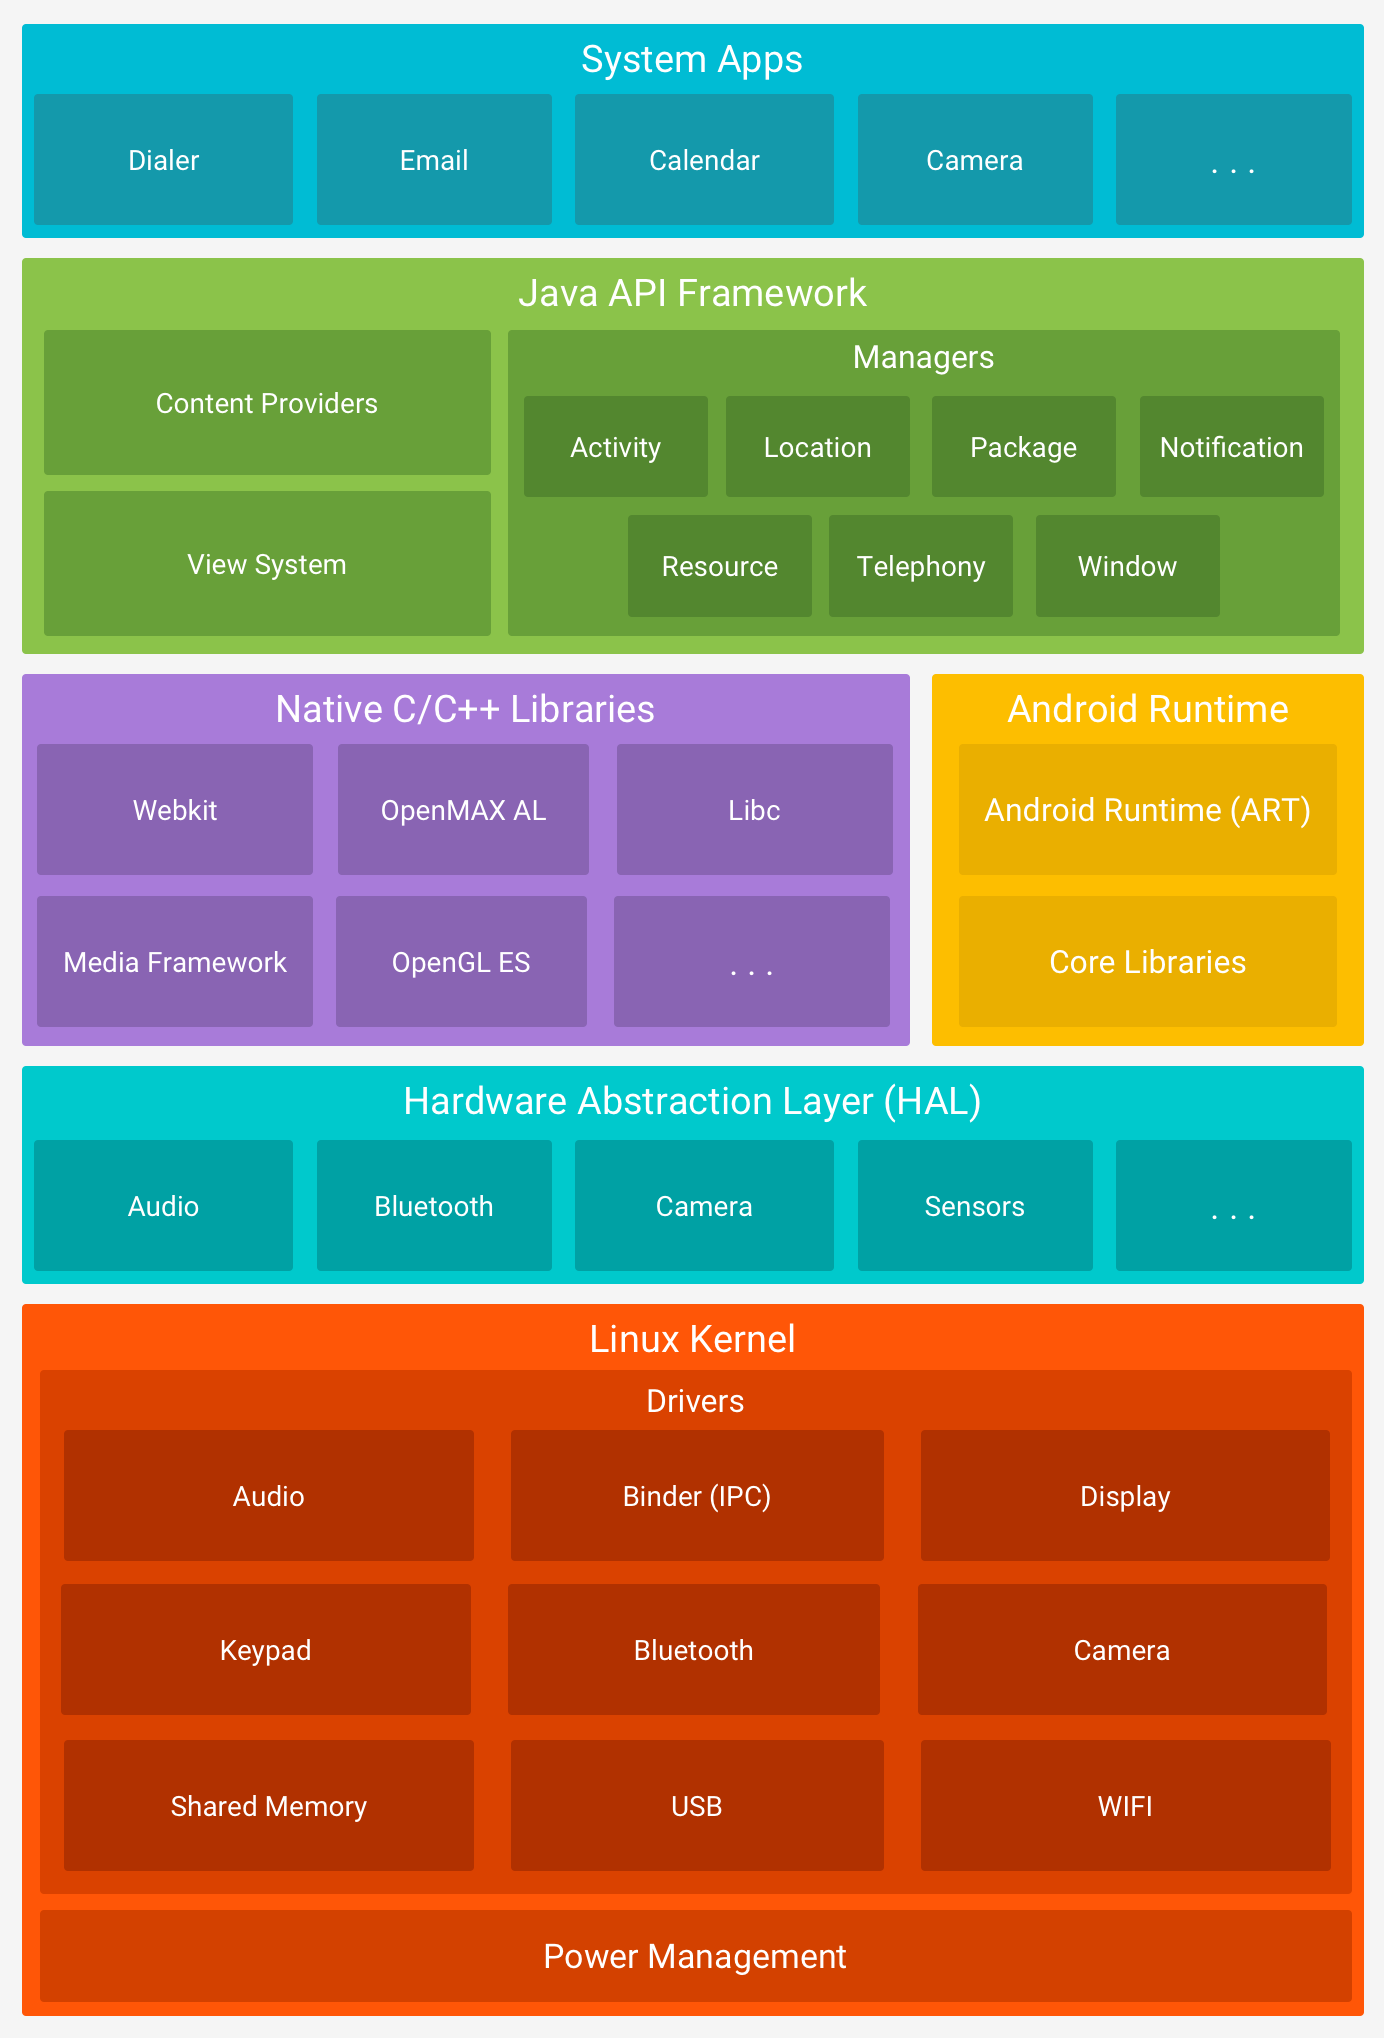
\includegraphics[width=12cm]{Imagens/arqandroid.png} 
    \caption{Arquitetura do Android}
    \label{android}
    \cite{Doc2024}
    \end{figure}

    
    \subsection{Componentes do android}
    Segundo \citeonline{Elenkov2014}, os aplicativos Android são uma combinação de componentes fracamente acoplados e com vários pontos de acesso. Cada componente pode oferecer vários pontos de entrada que podem ser alcançados com base nas ações do usuário no mesmo ou em outro aplicativo, ou acionados por um evento do sistema sobre o qual o aplicativo registrou para ser notificado.

    Os componentes são definidos no arquivo manifesto do aplicativo, chamado AndroidManifest.xml, que é um arquivo que descreve informações essenciais sobre a aplicação para as ferramentas de build do Android, para o sistema operacional Android e para o Google Play. 
    
    Os componentes principais e descritos por \citeonline{Elenkov2014} são:

    \subsubsection{Activities}
    Uma activity é uma tela única com uma interface de usuário. Elas são os principais blocos de construção dos aplicativos da GUI do Android. Um aplicativo pode ter várias atividades e, embora geralmente sejam projetadas para serem exibidas em uma ordem específica, cada atividade pode ser iniciada de forma independente, potencialmente por um aplicativo diferente (se permitido).
    
    \subsubsection{Services}
    Um service é um componente executado em segundo plano e não tem interface de usuário. Esses componentes são normalmente usados para executar alguma operação de longa duração, como baixar um arquivo ou reproduzir música, sem bloquear a interface de usuário. Eles também podem definir uma interface remota e fornecer alguma funcionalidade para outros aplicativos. No entanto, diferentemente dos serviços do sistema, que fazem parte do sistema operacional e estão sempre em execução, os serviços do aplicativo são iniciados e interrompidos sob demanda.
    
    \subsubsection{Content providers}
    Os content providers fornecem uma interface para dados do aplicativo, que normalmente são armazenados em um banco de dados ou arquivos. Eles podem ser acessados via comunicação entre processos e são usados principalmente para compartilhar os dados de um aplicativo com outros aplicativos. Os content providers oferecem controle refinado sobre quais partes dos dados são acessíveis, permitindo que um aplicativo compartilhe apenas um subconjunto de seus dados.
    
    \subsubsection{Broadcast receivers}
    Um broadcast receivers é um componente que responde a eventos de todo o sistema, chamados transmissões. As transmissões podem se originar do sistema (por exemplo, anunciando alterações na conectividade de rede) ou de um aplicativo de usuário (por exemplo, anunciando que a atualização de dados em segundo plano foi concluída).
    
    \subsection{Mecanismos de segurança do sistema operacional}
    \label{mecanismos}
    De acordo com \citeonline{Doc2024}, o Android incorpora diversos mecanismos de segurança destinados a proteger o sistema e os dados do usuário contra ameaças e ataques. \citeonline{Stevenson2021} descreve alguns deles: 

    \subsubsection{Sandboxing}
    O Android atribui automaticamente um identificador de usuário único, frequentemente chamado de ID de aplicativo, a cada aplicação no momento da instalação e executa essa aplicação em um processo dedicado rodando com aquele identificador. Assim, as aplicações são isoladas ou colocadas em sandbox, isso é, um ambiente de computação controlado que permite a realização de ações de forma privativa, sem riscos, interferências e modificações externas; tanto no nível do processo quanto no nível de arquivos. 
    
    \subsubsection{Permissões}
    Como as aplicações Android são isoladas em sandboxs, elas só podem acessar seus próprios arquivos e quaisquer recursos do dispositivo que sejam acessíveis a todos. Contudo, uma aplicação com tais restrições não seria muito interessante. Para permitir uma funcionalidade mais rica, o Android pode conceder direitos de acesso adicionais e mais detalhados às aplicações. Esses direitos de acesso são chamados de permissões.

    De maneira simples, uma permissão é simplesmente uma string que denota a capacidade de executar uma operação específica. A operação de destino pode ser coisas desde acessar um recurso físico ou dados compartilhados até a capacidade de iniciar ou acessar um componente em um aplicativo de terceiros. Definir parâmetros como  \textbf{protectionLevel} = ``signature'' (permite apenas aplicações assinadas da mesma forma de acessar o componente) e  \textbf{permission} = ``android .permission.READ\_PROVIDER'' (permite apenas a leitura de informações do componente), são algumas formas de exigir permissões para acessar componentes de uma aplicação
    
    \subsubsection{IPC}
    A comunicação entre processos ou Inter-Process Communication (IPC) no Android é um aspecto crucial do desenvolvimento de aplicações, permitindo que componentes de diferentes aplicações ou de diferentes partes de uma mesma aplicação possam interagir de maneira segura e eficiente. O Android oferece várias ferramentas e mecanismos para facilitar essa comunicação; como Intents e exportação de componentes. Os mecanismos de IPC do Android permitem conferir a identidade do aplicativo que está se conectando à sua IPC e definir políticas de segurança para cada mecanismo.

    \subsubsubsection{Intent}
    Uma Intent é uma descrição abstrata de uma operação a ser realizada. Ela pode ser usada para iniciar um Activity, solicitar informação a um Content Provider ou para se comunicar com um Service. Elas fornecem recursos para executar vinculação tardia de tempo de execução entre o código em diferentes aplicativos. Seu uso mais significativo é no lançamento de atividades, onde pode ser pensado como a cola entre as atividades. É basicamente uma estrutura de dados passiva que contém uma descrição abstrata de uma ação a ser executada.

    \subsubsubsection{Componentes exportados}]
    O Android desenvolveu um parâmetro chamado \textbf{exported}, que define se um componente pode ser iniciado por componentes de outros aplicativos ou não:

    Se \textbf{True}, qualquer aplicativo pode acessar a atividade e iniciá-la pelo nome exato da classe.
    
    Se \textbf{False}, somente componentes do mesmo aplicativo, aplicativos com o mesmo ID de usuário ou componentes de sistema privilegiados podem realizar ações.

    \subsubsection{Desafios de segurança}
    Segundo \citeonline{Hermans2023}, apesar desses robustos mecanismos de segurança, o Android enfrenta vários desafios devido à sua natureza aberta e à fragmentação do ecossistema. A diversidade de dispositivos e versões do Android pode dificultar a distribuição uniforme de atualizações de segurança, deixando alguns dispositivos vulneráveis por longos períodos. A abertura do ecossistema permite que desenvolvedores distribuam aplicações fora da Google Play Store, aumentando o risco de instalação de aplicativos maliciosos. Ademais, os fabricantes de dispositivos podem modificar o Android, potencialmente introduzindo novas vulnerabilidades ou dificultando a aplicação de patches de segurança padrão. Além dos desafios sistêmicos, as vulnerabilidades a nível de aplicação, citadas na seção \ref{owasp}, também representam uma ameaça significativa à segurança no Android. 
    
    \section{Vulnerabilidades, ameaças, riscos e exposição}
    \citeonline{Garg2023} classificam vulnerabilidades como defeitos de segurança suscetíveis a exploração, podendo comprometer os pilares da segurança de um sistema. Estas fragilidades podem se manifestar em diferentes camadas, desde falhas de software até configurações inadequadas e podem ser utilizadas para crimes cibernéticos, para violar a sua privacidade, perturbar a infraestrutura e criar riscos para a segurança nacional. Identificar, corrigir, evitar e principalmente conhecer essas vulnerabilidades é crucial para mitigar riscos e garantir que sistemas permaneçam resilientes diante de potenciais ameaças.
    
    \subsection{OWASP Mobile Top 10 2023 e ciberataques}
    \label{owasp}
    
    O OWASP Mobile Top 10, vista na tabela \ref{tab:owasptt}, é uma lista das principais ameaças e vulnerabilidades de segurança encontradas em aplicações móveis. É um guia elaborado pela organização Open Web Application Security Project (\citeonline{owasp2023}) e uma referência crucial para desenvolvedores, arquitetos de segurança, avaliadores de segurança e quaisquer profissional envolvido com segurança ou desenvolvimento de aplicações mobile. 

    \begin{table}[H]
    \centering
    \caption{OWASP Mobile Top 10 2024}
    \label{tab:owasptt}
    \begin{tabular}{|l|}
    \hline
    \rowcolor[HTML]{68CBD0} 
    \multicolumn{1}{|c|}{\cellcolor[HTML]{68CBD0}{\color[HTML]{FFFFFF} \textbf{OWASP Mobile Top 10 2024: Final Release Updates}}} \\ \hline
    M1: Uso impróprio de credenciais                                                                                              \\ \hline
    M2: Segurança inadequada da cadeia de suprimentos                                                                             \\ \hline
    M3: Autenticação/Autorização Insegura                                                                                         \\ \hline
    M4: Validação de entrada/saída insuficiente                                                                                   \\ \hline
    M5: Comunicação Insegura                                                                                                      \\ \hline
    M6: Controles de privacidade inadequados                                                                                      \\ \hline
    M7: Proteções binárias insuficientes                                                                                          \\ \hline
    M8: Configuração incorreta de segurança                                                                                       \\ \hline
    M9: Armazenamento de dados inseguro                                                                                           \\ \hline
    M10: Criptografia insuficiente                                                                                                \\ \hline
    \end{tabular}
    \end{table}
    
    
    A lista, citada acima, identifica e descreve as vulnerabilidades mais comuns e críticas que são encontradas e exploradas em aplicativos móveis, abrangendo desde questões de autenticação e autorização até problemas relacionados à criptografia e gestão de sessões. O OWASP Mobile Top 10 não apenas destaca os desafios de segurança enfrentados pelas aplicações móveis, mas também orienta a comunidade de desenvolvimento na adoção de boas práticas e na implementação de métodos de segurança eficazes contra estas vulnerabilidades. O guia é atualizado frequentemente, tendo como ultima atualização a de 2023, para acompanhar as mudanças no cenário de ameaças, garantindo que os profissionais estejam sempre atualizados e equipados para enfrentar os desafios emergentes na segurança de aplicações móveis. Segundo a própria organização, as vulnerabilidades são descritas em \cite{owasp2023}.
    
     
    \section{Aplicações Bancárias}
    \label{bancos}
    
    Os serviços bancários móveis compartilham as necessidades críticas de segurança da informação de outros aplicativos, mas diferem em alguns aspectos de implementação e preocupações específicas \cite{Ahmad2015}.
    
    \subsection{Desafios, ameaças e remediações}
    
    Todos os tipos de sistemas são alvos de criminosos cibernéticos. Por conta disso, muitas ameaças diferentes são encontradas e mecanismos de segurança são adotados para garantir a segurança dos sistemas.

    Dessa forma foi realizada uma revisão na literatura com o objetivo de encontrar as mais críticas ameaças e vulnerabilidades encontradas nas aplicações bancárias e suas respectivas remediações e soluções. Resultando nas informações compiladas na seguinte tabela \ref{tab:vuln}: 
    

    \begin{table}[H]
    \centering
    \caption{Principais vulnerabilidades em aplicações bancárias}
    \label{tab:vuln}
    \begin{tabular}{|p{5cm}|p{5cm}|p{5cm}|}
    \hline
    \textbf{Referência} & \textbf{Vulnerabilidades e Ameaças} & \textbf{Soluções e Remediações} \\ \hline
    
    \citeonline{Chen2020} & Vulnerabilidades relacionadas a criptografia imprópria, autenticação inválida e armazenamento inseguro. & Proposta de AUSERA para identificar vulnerabilidades; boas práticas em criptografia e autenticação. \\ \hline
    
    \citeonline{Yildirim20219} & Falhas de dispositivo (permissões, armazenamento de dados e senhas fracas), Rede (MITM e problemas de criptografia) e Data Center (injeção de código). & Uso correto de criptografia, certificados digitais, autenticação multifator (2FA), gerenciamento de sessões e CAPTCHA. \\ \hline
    
    \citeonline{Darem2023} & Phishing, malware, DDoS, ataques man-in-the-middle, ataques de senha e computação quântica. & Criptografia de dados em repouso e em trânsito, segmentação de rede, firewalls, IPS, autenticação multifator, e políticas legais e organizacionais. \\ \hline
    
    \citeonline{Ubaldo2023} & Malwares, Phishing, violações de dados, DoS e XSS. & Biometria, conscientização sobre phishing, tokens de software e hardware, investimento contínuo em cibersegurança. \\ \hline
    
    \citeonline{Chandra2023} & Dados não criptografados, malware, serviços de terceiros, falsificação e Phishing. & Criptografia de dados, aplicativos antimalware, conscientização do consumidor. \\ \hline

    \end{tabular}
    \end{table}
    
    
    \begin{table}[H]
    \centering
    \begin{tabular}{|p{5cm}|p{5cm}|p{5cm}|}
    \hline
    
    \citeonline{falade2023} & Códigos e aplicações maliciosas, fraude, roubo de identidade, negação de serviço, Wi-Fi não criptografado, acesso não autorizado e perda de dispositivos. & Comportamento seguro dos usuários, governança e medidas técnicas de segurança em aplicativos. \\ \hline
    
    \citeonline{Alzoubi2022} & Dados não criptografados, malware, spoofing, manipulação de dados. & Certificados digitais, tokens OTP, monitoramento transacional, criptografia. \\ \hline
    
    \citeonline{Wodo2021} & Falhas de autenticação, Root/Jailbreak, redes inseguras. & MFA, proteção baseada em PIN/biometria, uso de redes seguras. \\ \hline
    
    \citeonline{Stanikzai2021} & Malware, ataques de negação de serviço, phishing, fraude, roubo de identidade. & Scanner de vulnerabilidade, IPS, gestão cíclica de cibersegurança e políticas de segurança documentadas. \\ \hline
    
    \citeonline{Boitan2019} & Roubo de dados, acesso não autorizado, phishing, interrupção de negócios. & Prevenção, identificação e gestão de incidentes cibernéticos no setor financeiro. \\ \hline
    
    \citeonline{Muhammad2023} & Phishing, malware, ataques de engenharia social, ameaças internas. & Mecanismos de autenticação seguros, criptografia moderna, canais de comunicação seguros e detecção de fraudes em tempo real. \\ \hline
    
    \citeonline{sota2020} & Riscos relacionados à autenticação e tokenização em pagamentos móveis. & Implementação de tokenização, protocolos seguros, autenticação multifator. \\ \hline
    
    \citeonline{Wang2016} & Malware, vazamento de informações, autenticação de maneira geral, vulnerabilidades de redes e certificados. & TLS, autenticação multifatorial, detecção e proteção contra fraudes e malware. \\ \hline
    
    \citeonline{Datta2020} & Crescimento de fraudes online no setor bancário. & Programas de conscientização entre clientes. \\ \hline
    
    \end{tabular}
    \end{table}

    \subsection{Principais vulnerabilidades levantadas}
    \label{ameaças}
    Os estudos abordados na revisão da literatura destacam vários tipos de vulnerabilidades e ameaças enfrentadas por essas plataformas, que comprometem a confidencialidade, integridade e disponibilidade dos dados dos usuários. 
    
    Dentre elas, as entendias mais críticas e recorrentes são:

    \subsubsection{Malwares}
    Malwares, por exemplo, representam uma das ameaças mais significativas para aplicações bancárias móveis. De acordo com pesquisas de \citeonline{Darem2023}, \citeonline{Chandra2023} e \citeonline{Alzoubi2022}, malwares são ameaças graves principalmente para plataformas bancárias e móveis, pois visam roubo de credenciais bancárias e dados pessoais e acesso a componentes sensíveis. Estes softwares maliciosos podem se infiltrar nos dispositivos dos usuários por meio de aplicativos falsos ou comprometidos, geralmente disfarçados como apps legítimos ou através de ataques de engenharia social.

    \subsubsection{Autenticação Insegura}
    Ataques de autenticação constituem outro risco crítico. O processo de autenticação é frequentemente alvo de ataques como força bruta, informações vazadas e exploração de vulnerabilidades de implementação, como citado por \citeonline{Chen2020} e \citeonline{sota2020}. Cibercriminosos tentam comprometer o processo de login dos usuários para obter acesso não autorizado às suas contas ou até mesmo realizar ações já estando logados na conta da vítima. Conforme destacado pelo \citeonline{owasp2023}, a autenticação inadequada é uma das principais falhas de segurança em aplicações móveis. 

    \subsubsection{Criptografia insuficiente}
    Como citado por \citeonline{Ubaldo2023} e \citeonline{falade2023}, a criptografia inadequada é um dos principais fatores críticos a se considerar durante a implementação, especialmente em aplicações que lidam com dados sensíveis como informações financeiras. A criptografia mal implementada pode ser vulnerável a ataques de força bruta, criptoanálise, ou até mesmo a falsificação, assim, expondo informações sensíveis dos usuários e possibilitando transações falsas.

    \subsubsection{Comunicação Insegura}
    Por fim, ataques de rede são uma ameaça constante para aplicações bancárias móveis, uma vez que a comunicação entre o cliente e o servidor pode ser interceptada ou manipulada. Segundo \citeonline{Yildirim20219}, ataques man-in-the-middle (MITM) são frequentes em aplicações bancárias móveis devido a mobilidade dos dispositivos que as implementam. 

    
    \subsection{Arquitetura de aplicações bancárias}
    
    A arquitetura do sistema desempenha um papel crucial na construção de plataformas financeiras digitais seguras, eficientes, confiáveis e centrados no usuário. Dessa forma, ela devem ser projetadas para garantir a segurança, escalabilidade e adaptabilidade às mudanças tecnológicas. No contexto de um banco móvel, a arquitetura geralmente compreende camadas distintas, incluindo o front-end, responsável pela interface do usuário intuitiva e acessível, o back-end que gerencia a lógica de negócios e a manipulação segura de dados, e a camada de segurança, incorporando autenticação robusta e criptografia para proteger a confidencialidade das informações financeiras dos usuários.

    \begin{figure}[H]
    \centering 
    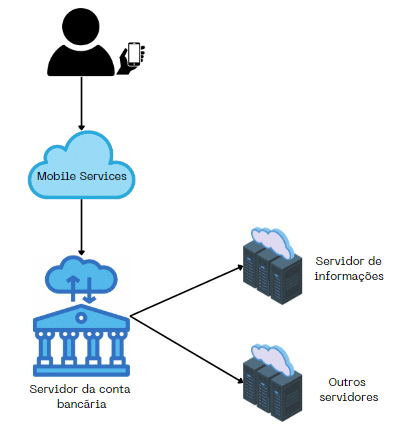
\includegraphics[width=6cm]{Imagens/arcB.png} 
    \caption{Arquitetura de uma aplicação de banco móvel}
    \label{arcB}
    \end{figure}
    
    Como proposto por \citeonline{Ahmad2015}, as aplicações bancárias móvel carregam uma arquitetura simples por conter apenas ações e validações internas da própria instituição, como pode-se ver na figura \ref{arcB}. O dispositivo utilizado, que é acessado pelo usuário para interagir com o sistema, exibi os menus e transmite mensagens curtas de forma segura. A plataforma do banco facilita a transferência de mensagens curtas para comandos bancários compatíveis. A interação entre o usuário e o provedor de serviços ocorre por meio de diálogos multiníveis, com o banco fornecendo suporte e executando instruções nas contas bancárias. O Sistema de banco móvel também suporta a comunicação com outros servidores contribuindo para a ampliação dos serviços oferecidos ao usuário.
    

    \subsection{PCI DSS}
    \label{pci}

    O Payment Card Industry Data Security Standard (PCI DSS) é um conjunto de normas de segurança criado com o objetivo de proteger os dados dos usuários de serviços de pagamento e assegurar que as empresas que processam, armazenam ou transmitem essas informações mantenham um ambiente seguro. Este padrão foi estabelecido pelo PCI Security Standards Council \cite{pci2022}, um fórum global independente formado em 2006 por grandes marcas de cartões de crédito, incluindo Visa, MasterCard, American Express, Discover e JCB, que colaboram para melhorar a segurança dos pagamentos em todo o mundo.
    
    Segundo \citeonline{Seaman2020}, e seu uso é obrigatório pelas marcas de cartão, o que a torna uma das certificações de segurança internacional mais reconhecidas do mercado de pagamentos. O método de avaliação é aplicado a qualquer empresa que processe, armazene ou transmita dados de cartões de crédito e débito, independentemente do tamanho da organização ou do volume de transações processadas. Empresas que não se adéquam às normas estão sujeitas a receberem multas e até mesmo a serem descredenciadas junto às operadoras e bandeiras de cartão de crédito.

    \subsubsection{Requisitos da certificação}
    Para estar em conformidade com o PCI DSS, todas as empresas devem atender a 12 requisitos básicos, organizados em 6 categorias abrangentes que cobrem desde a construção e manutenção de uma rede segura até a implementação de políticas robustas de segurança da informação, conforme descrito pela \citeonline{pci2022}:
    
    \begin{enumerate}
        \item Construir e manter uma rede e sistemas seguros
            \begin{enumerate}
            \item Instalar e manter controles de segurança de rede. 
            \item Aplicar as configurações de segurança para todos os componentes de sistema.
            \end{enumerate}

        \item Proteger os dados da conta
            \begin{enumerate}
            \item Proteger os dados da conta armazenados.
            \item Proteger os dados do titular do cartão com criptografia forte durante a transmissão em redes públicas abertas.
            \end{enumerate}

        \item Manter um programa de gestão de vulnerabilidade
            \begin{enumerate}
            \item Proteger todos os sistemas e redes de software malicioso.
            \item Desenvolver e manter sistemas e software seguros.
            \end{enumerate}

        \item Implementar medidas fortes de controle de acesso
            \begin{enumerate}
            \item Restringir o acesso aos componentes de sistema e aos dados do titular do cartão por necessidade de conhecimento do negócio.
            \item Identificar usuários e autenticar o acesso aos componentes de sistema
            \item Restringir o acesso físico aos dados do titular do cartão.
            \end{enumerate}

        \item Monitorar e testar as redes regularmente
            \begin{enumerate}
            \item Registrar e monitorar todo o acesso aos componentes de sistema e dados do titular do cartão.
            \item Testar a segurança de sistemas e redes regularmente.
            \end{enumerate}

        \item Manter uma política de segurança da informação
            \begin{enumerate}
            \item Apoiar a segurança da informação com políticas e programas organizacionais.
            \end{enumerate}
    \end{enumerate}

    \subsubsection{Importância do PCI DSS}
    A importância do PCI DSS vai além do simples cumprimento de uma norma de segurança; ele é um pilar fundamental para a proteção das transações financeiras em um mundo cada vez mais digitalizado. A conformidade com o PCI DSS ajuda a prevenir a exposição de informações sensíveis dos titulares de cartões, reduzindo significativamente o risco de fraudes e violações de dados. Considerando o volume de transações realizadas diariamente, uma falha de segurança pode ter consequências catastróficas, tanto financeiras quanto reputacionais, para as empresas envolvidas.

    A conformidade com o PCI DSS também facilita a criação de um ambiente de segurança robusto dentro da organização. Ao seguir as diretrizes estabelecidas pelo padrão, as empresas desenvolvem uma cultura de segurança da informação que permeia toda a sua estrutura. Isso não só protege os dados dos titulares de cartões, mas também fortalece as defesas contra outros tipos de ameaças cibernéticas, como ataques de malware e violações internas. A implementação contínua dessas práticas de segurança ajuda a garantir que as empresas estejam melhor preparadas para enfrentar novos desafios no cenário de cibersegurança.

    No contexto regulatório, o PCI DSS serve como uma base para o cumprimento de outras normativas e leis de proteção de dados, como o General Data Protection Regulation (GDPR) na Europa e a Lei Geral de Proteção de Dados (LGPD) no Brasil. Embora o PCI DSS seja específico para o setor de pagamentos, sua implementação pode ser um passo inicial para a conformidade com esses outros regulamentos, criando uma sinergia entre as diferentes exigências legais.
    
    \section{Engenharia de Requisitos}
    Segundo \citeonline{Pohl2015}, os requisitos de um sistema são descrições das funcionalidades que o sistema deve possuir, os serviços que ele oferece e condições ou capacidades que deve ser atendida ou possuídas pelo mesmo. Esses requisitos refletem as necessidades dos clientes para um sistema que atende a uma finalidade específica,  quais são suas demandas e dores e o que é necessário para solucioná-la, dentro do que está sendo proposto. O processo de descobrir, analisar, documentar e verificar esses serviços e restrições é conhecido como engenharia de requisitos. 
    
    Os requisitos de software são frequentemente classificados como requisitos funcionais e requisitos não funcionais:
    
    \subsection{Requisitos funcionais}
    Os requisitos funcionais de um sistema descrevem as funcionalidades que ele deve executar. Esses requisitos variam conforme o tipo de software a ser desenvolvido, seus possíveis usuários e a abordagem adotada pela organização ao redigir os requisitos. Quando expressos como requisitos de usuário, são normalmente descritos de maneira abstrata, para garantir a compreensão pelos usuários do sistema. No entanto, requisitos funcionais de sistema mais específicos detalham as funções do sistema, suas entradas e saídas, e as exceções. Esses requisitos podem variar de descrições gerais, que abrangem as principais funcionalidades do sistema, até especificações muito detalhadas, que refletem as operações e processos específicos de uma organização.
    
    \subsection{Requisitos não funcionais}
    Os requisitos não funcionais são aqueles que não estão diretamente ligados aos serviços específicos que o sistema oferece aos seus usuários. Eles se relacionam às propriedades emergentes do sistema, como confiabilidade, tempo de resposta e uso de recursos. Esses requisitos normalmente especificam ou restringem as características do sistema como um todo, como mostrado na figura \ref{naofunc}, o que os torna frequentemente mais críticos que requisitos funcionais individuais.
    
    
    \subsubsection{Requisitos de segurança}
    De acordo com \citeonline{Dalpiaz2016}, requisitos de segurança constituem um conjunto de diretrizes, normas e práticas essenciais para assegurar a proteção de um sistema ou ambiente. Esses requisitos são desenvolvidos a partir de análises de risco detalhadas, levando em conta as possíveis ameaças que poderiam comprometer a segurança dos ativos de uma organização e podem ser classificados em várias categorias principais, como autenticação, autorização, confidencialidade, integridade, disponibilidade, conscientização e treinamento, cada um com seu papel e importância na implementação e uso seguro de sistemas de informação.

    \begin{figure}[H]
    \centering 
    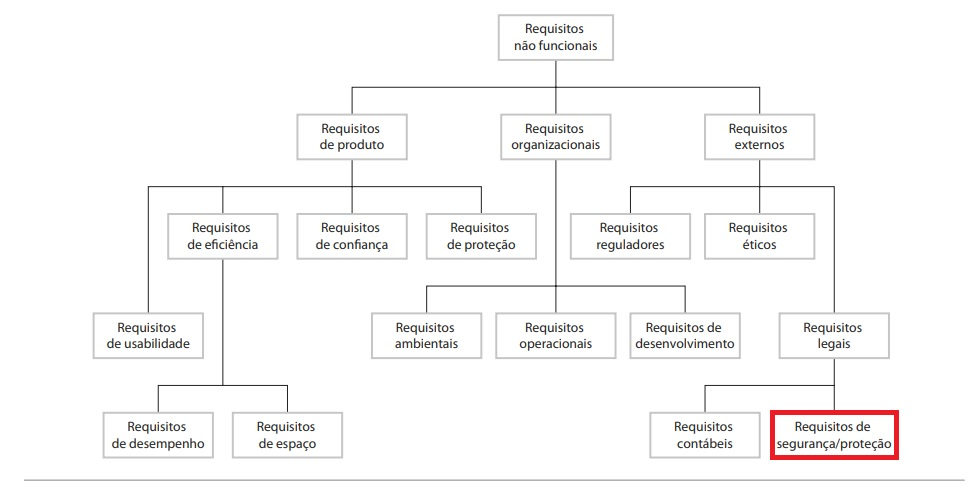
\includegraphics[width = 16cm]{Imagens/naofucnionais.jpg}
    \caption{Tipos de requisitos não funcionais}
    \cite{sommerville2011}
    \label{naofunc}
    \end{figure}
    
    Definir requisitos de segurança eficazes pode ser desafiador devido à complexidade dos sistemas modernos e à diversidade das ameaças, como vemos na seção  \ref{owasp}. Requisitos de segurança devem ser claros, mensuráveis e verificáveis. Eles também precisam ser adaptáveis para evoluir com as novas ameaças e tecnologias emergentes.
    
    
    \subsection{Ciclo de vida da Engenharia de requisitos}
    
    A Engenharia de Requisitos envolve várias fases que se repetem em um ciclo contínuo: Estudo de Viabilidade, Elicitação, Modelagem e Análise, Validação e Gerenciamento. Durante o desenvolvimento e a manutenção do software, essas etapas são continuamente realizadas para analisar os problemas e as necessidades do projeto, oferecendo soluções baseadas nos requisitos definidos. Esse ciclo é baseado nas atividades definidas e descritas por \citeonline{sommerville2011}.
    
    \subsubsection{Estudo de Viabilidade}
    O ciclo de vida da engenharia de requisitos começa com o Estudo de Viabilidade, uma fase crucial para determinar a viabilidade técnica, econômica e operacional do projeto. Nesta etapa, os analistas de sistemas realizam uma série de investigações para avaliar se os requisitos iniciais podem ser satisfeitos dentro das restrições de recursos, tempo e tecnologia disponíveis. É uma análise abrangente que busca responder a perguntas fundamentais como: "É tecnicamente possível desenvolver este sistema?", "Os benefícios superam os custos?", e "A organização está preparada para adotar essa solução?". Esta fase também envolve a identificação de possíveis riscos e a definição de estratégias para mitigá-los, ajudando a decidir se o projeto deve avançar, ser modificado ou mesmo abandonado.
    
    \subsubsection{Elicitação}
    Após a viabilidade do projeto ser confirmada, inicia-se a etapa de Elicitação de Requisitos, onde se busca compreender as necessidades e expectativas dos usuários e das partes interessadas. Esta fase é fundamental para garantir que os requisitos coletados sejam completos e representativos das verdadeiras necessidades do negócio. Diversas técnicas são empregadas para coletar essas informações, incluindo entrevistas, questionários, workshops, observações diretas, e análise de documentos existentes. A elicitação é um processo interativo que exige comunicação eficaz e colaboração entre os analistas de sistemas e os stakeholders. O objetivo é assegurar que todos os requisitos relevantes sejam identificados e compreendidos.
    
    \subsubsection{Modelagem e Análise}
    Com os requisitos coletados, a próxima etapa é a Modelagem e Análise. Nesta fase, os requisitos são organizados e representados de maneira estruturada, utilizando ferramentas de modelagem como diagramas de casos de uso, diagramas de atividades e modelagem de processos. Estas representações visuais ajudam a clarificar os requisitos, identificar lacunas, redundâncias e possíveis conflitos. A análise dos requisitos também envolve a verificação de sua completude, consistência e viabilidade. É nesta fase que os requisitos são refinados e detalhados, assegurando que estejam claros e compreensíveis tanto para a equipe técnica quanto para os stakeholders.
    
    \subsubsection{Validação}
    Uma vez modelados e analisados, os requisitos devem ser validados. A Validação é a etapa onde se verifica se os requisitos realmente refletem as necessidades e expectativas dos usuários e se são viáveis do ponto de vista técnico. Esta fase pode envolver revisões de requisitos, prototipagem, simulações e testes de requisitos para garantir que os requisitos são corretos e completos. A validação é um processo colaborativo que envolve revisões com as partes interessadas para confirmar que o sistema desenvolvido atenderá às suas expectativas e requisitos. O objetivo é garantir a qualidade e a aderência dos requisitos às necessidades reais do projeto.
    
    \subsubsection{Gerenciamento}
    Por fim, a etapa de Gerenciamento de Requisitos é um processo contínuo que se estende por todo o ciclo de vida do projeto. O gerenciamento de requisitos envolve a rastreabilidade, controle de versões e controle de mudanças nos requisitos. Ferramentas e técnicas de gerenciamento são utilizadas para manter a documentação atualizada, avaliar o impacto de alterações nos requisitos e comunicar essas mudanças às partes interessadas. Esta etapa é crucial para manter a integridade e consistência dos requisitos ao longo do desenvolvimento do sistema, garantindo que todas as mudanças sejam aprovadas e documentadas adequadamente.
    
    
    \subsection{Importância da engenharia de requisitos na segurança}

    A engenharia de requisitos desempenha um papel fundamental na segurança da informação, pois estabelece as bases sobre as quais sistemas seguros são construídos. Segundo  \citeonline{Dalpiaz2016}, a definição precisa e clara dos requisitos de segurança é essencial para antecipar e mitigar possíveis ameaças e vulnerabilidades que possam comprometer a integridade, confidencialidade e disponibilidade dos dados. Sem uma sólida engenharia de requisitos, os sistemas correm o risco de apresentar brechas que podem ser exploradas por agentes maliciosos, resultando em perdas financeiras, danos à reputação e outras consequências graves.

    Um dos principais aspectos da engenharia de requisitos na segurança da informação é a capacidade de identificar e entender as ameaças e riscos específicos ao contexto do sistema em desenvolvimento. Ao envolver todas as partes interessadas, incluindo analistas de segurança, desenvolvedores, e usuários finais, a engenharia de requisitos garante que todas as perspectivas sejam consideradas. Este processo colaborativo é crucial para a identificação de possíveis pontos fracos e para a definição de medidas de segurança que sejam práticas e eficazes no contexto operacional real do sistema.
    
    A engenharia de requisitos também é vital para a integração de segurança ao longo de todo o ciclo de vida do desenvolvimento de software. Ao definir claramente os requisitos de segurança desde as fases iniciais, é possível incorporar práticas de segurança em cada etapa do desenvolvimento, desde o design até a implementação e testes. Isso não só aumenta a robustez do sistema contra ataques, mas também reduz os custos associados à correção de falhas de segurança descobertas em estágios mais avançados, onde tais correções são tipicamente mais dispendiosas e complexas.
    
    Além disso, a documentação precisa e detalhada dos requisitos de segurança facilita a comunicação e o entendimento entre todos os membros da equipe de desenvolvimento. Ela serve como uma referência clara para desenvolvedores, testadores e auditores, garantindo que todos estejam cientes das exigências de segurança e das justificativas por trás de cada medida implementada. Isso promove uma cultura de segurança dentro da organização, onde a proteção dos dados é vista como uma responsabilidade compartilhada.
    

    \section{Modelos e padrões de segurança para aplicações móveis}
    As aplicações móveis enfrentam diversas ameaças de segurança, sendo essencial a adoção de diretrizes robustos para mitigar esses riscos. Estes modelos e padrões são fundamentais para o desenvolvimento de aplicações móveis seguras, oferecendo diretrizes claras e práticas recomendadas para enfrentar os desafios de segurança específicos deste ambiente. Ao aderir a estes padrões, desenvolvedores e organizações podem melhorar significativamente a segurança de suas aplicações móveis, protegendo os dados dos usuários e garantindo a integridade e a confiabilidade dos serviços oferecidos.

    \subsection{OWASP MASVS}
    O OWASP Mobile Application Security Verification Standard (MASVS) \cite{masvs2019} é um padrão globalmente reconhecido para a segurança de aplicações móveis. Ele fornece um conjunto de requisitos de segurança que podem ser utilizados como base para avaliar a segurança de uma aplicação móvel. O MASVS é dividido em várias categorias, incluindo arquitetura de segurança, manipulação de dados, autenticação, gerenciamento de sessão, criptografia e comunicação. Cada categoria contém requisitos específicos que devem ser atendidos para garantir a segurança da aplicação. O objetivo do MASVS é ajudar desenvolvedores, testadores de segurança e arquitetos a garantir que as aplicações móveis sejam desenvolvidas e testadas de acordo com as melhores práticas de segurança.
    
    \subsection{NIST SP 800-163}
    O NIST Special Publication 800-163 \cite{Ogata2019} fornece diretrizes detalhadas para a avaliação da segurança de aplicações móveis. Este documento aborda o processo de verificação de segurança, incluindo a identificação de ameaças e vulnerabilidades, avaliação de riscos e implementação de controles de segurança. O NIST SP 800-163 destaca a importância de um processo contínuo de avaliação, recomendando práticas como análises estáticas e dinâmicas de código, testes de penetração e revisões de segurança de terceiros. Este padrão é amplamente utilizado por organizações governamentais e privadas nos Estados Unidos para garantir que as aplicações móveis estejam protegidas contra ameaças emergentes.

    \subsection{ISO/IEC 27034} 
    A ISO/IEC 27034 \cite{iso2018} é um padrão internacional que aborda a segurança de aplicações, incluindo aplicações móveis, no contexto do ciclo de vida do desenvolvimento de software. Este padrão fornece um framework abrangente para integrar práticas de segurança em todas as fases do desenvolvimento, desde o planejamento até a implementação e manutenção. A ISO/IEC 27034 enfatiza a importância de uma abordagem baseada em riscos, onde a segurança é adaptada às necessidades específicas da aplicação e do ambiente operacional. Além disso, o padrão define um conjunto de controles de segurança que podem ser aplicados para mitigar riscos específicos, promovendo a criação de aplicações mais seguras e resilientes.

    \chapter{Metodologia da Pesquisa}

    Este trabalho se inicia em uma revisão das literaturas, com o uso de diferentes trabalhos publicados em livros, revistas, periódicos e outros, para que sirva de base para suas análises. Por seguinte foram realizadas etapas do ciclo de vida da engenharia de requisitos a fim de se obter um modelo de segurança específico para aplicações bancárias no Android.

    Na Fig \ref{metodologia} mostraremos as etapas de como executaremos a apresentação do modelo proposto. Cada etapa será discutida em detalhes, evidenciando procedimentos realizados e as técnicas implementadas para garantir a integridade, confidencialidade e disponibilidade das informações no ambiente bancário.

    \begin{figure}[H]
    \centering 
    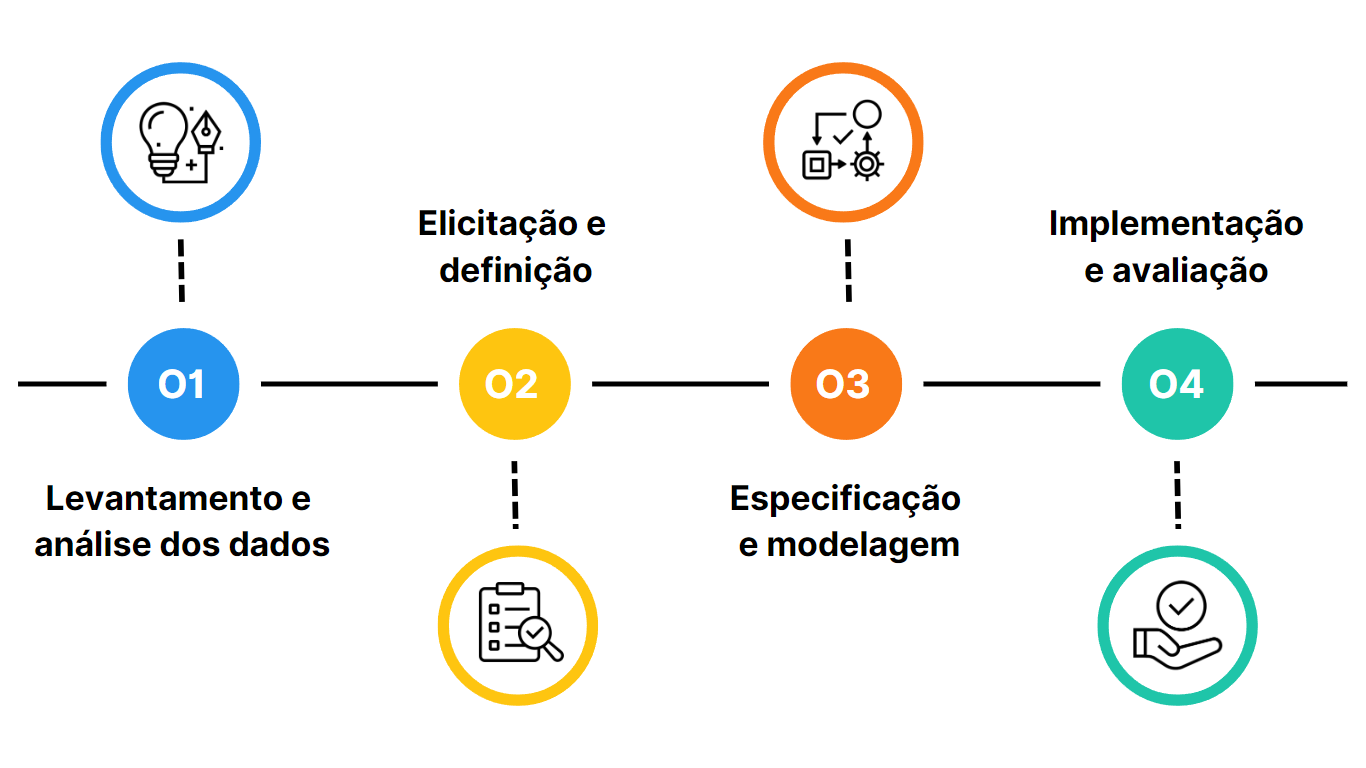
\includegraphics[width = 16cm]{Imagens/metodologia.png}
    \caption{Etapas adotada no trabalho}
    \label{metodologia}
    \end{figure}

    
    \section{Levantamento e análise de dados}
    Para a confecção do presente trabalho foram utilizados artigos científicos encontrados em plataformas públicas como Google Scholar, IEEE Xplore e Typeset.io por meio das palavras chave ``Mobile Banking Security'' e com a data da publicação entre os anos de 2019 e 2024. Como questões da pesquisa foram escolhidas as seguintes perguntas:

    \begin{itemize}[topsep=3pt, partopsep=3pt, itemsep=3pt, parsep=3pt]
        \item Quais são as ameaças de segurança mais críticas do setor bancário no android? 
        \item Quais são os métodos de segurança mais eficazes e viáveis para combater essas ameaças?
    \end{itemize}
    
    Com isso, foram selecionados artigos científicos com conteúdo técnico voltado ao pesquisador e desenvolvedor de aplicações bancárias com foco em segurança da informação, publicados em língua inglesa e com texto completo disponível. Dessa forma, evitando artigos não relacionados ao tema, incompletos, não publicados em língua inglesa e com conteúdo não técnico, isso é, artigos para usuários. Por fim, optou-se por incluir apenas artigos que ajudariam a responder as questão de pesquisa com base em uma leitura exploratória e análise de seu título, palavras-chave e resumo.

    Após a coleta dos dados, procedeu-se à leitura analítica do material, chegando na compilação das informações mais relevantes. Em seguida, foi conduzida uma análise descritiva, que visou não apenas compreender, mas também aprofundar o conhecimento sobre o tema investigado. Essa análise permitiu identificar padrões e tendências nos dados, contribuindo para a construção de um referencial teórico robusto e fundamentado, essencial para a compreensão aprofundada da segurança em aplicações bancárias móveis.

    \section{Elicitação e definição de requisitos de segurança utilizando a técnicas de casos de uso indevido}
    Com o compilado de informações, foi feita a elicitação dos requisitos utilizando a técnica de caso de uso indevido visando entender e descrever as principais interações maliciosas que podem comprometer o sistema e criar uma base para a definição dos requisitos de segurança.
    
    A técnica de casos de uso indevido é uma abordagem que pode ser utilizada na elicitação de requisitos de segurança ao identificar potenciais ameaças e vulnerabilidades que podem comprometer um sistema. Diferente dos casos de uso tradicionais, que descrevem interações desejadas entre usuários e o sistema, os casos de uso indevido focam em interações maliciosas que podem ser realizadas por atacantes para explorar fraquezas no sistema, isto é, as ameaças.

    Com a identificação dos casos de uso indevidos do sistema durante a revisão de literatura, foram definidos requisitos de segurança que especificam controles e mecanismos necessários para mitigar os riscos associados.

    \section{Especificação e modelagem dos requisitos de segurança utilizando diagramas UML}
    Após a elicitação dos requisitos de segurança, foi realizada a especificação e modelagem desses requisitos utilizando diagramas Unified Modeling Language (UML), para representar, organizar e comunicar os aspectos estruturais (estáticos) e comportamentais (dinâmicos) de um sistema de maneira clara e estruturada.

    Para este trabalho, utilizamos o software Visual Paradigm para criar diversos tipos de diagramas UML, incluindo:

    \begin{itemize}[topsep=3pt, partopsep=3pt, itemsep=3pt, parsep=3pt]
        \item Diagramas de Caso de Uso: Representam as interações entre os atores (usuários e sistemas externos) e o sistema, incluindo os casos de uso indevido identificados na fase anterior.
        \item Diagramas de Classe: Mostram como são implementadas as classes dentro do sistema, destacando os pontos onde os requisitos de segurança devem ser aplicados.
        \item Diagramas de Sequência: Ilustram a sequência de mensagens trocadas ou ações realizadas entre os componentes do sistema para cumprir os requisitos de segurança. 
    \end{itemize}
    
    Esses diagramas ajudam a visualizar como os requisitos de segurança se integram com os outros requisitos funcionais do sistema e a identificar possíveis inconsistências ou lacunas. A modelagem também facilita a comunicação e garante um entendimento comum dos requisitos de segurança.

    \section{Estudo de caso e avaliação do modelo}
    A etapa final do processo é um estudo de caso no qual os requisitos de segurança são propostos no ambiente Android, utilizando a aplicação bancária Herd Financial como base. O estudo de caso envolve a demonstração dos casos de uso do modelo de requisitos na aplicação bancária controlada. 

    Este estudo de caso permitiu validar a viabilidade técnica dos requisitos de segurança e testar sua eficácia em um cenário realista. Ao propor medidas de segurança diretamente à aplicação Herd Financial, foi possível observar como os controles de segurança poderiam interagir e se complementar no contexto de uma aplicação bancária. Além disso, este processo forneceu exemplos práticos de como os controles de segurança podem ser incorporados ao código-fonte do aplicativo Android, oferecendo uma referência valiosa para desenvolvedores que buscam implementar práticas de segurança semelhantes em suas próprias aplicações.

    Além disso, uma avaliação detalhada do modelo de segurança proposto para aplicações bancárias no Android, utilizando como referência a certificação PCI DSS. Esta certificação, desenvolvida pela PCI Security Standards Council, é amplamente reconhecida e exigida pelas principais bandeiras de cartão de crédito. A conformidade com os 12 requisitos fundamentais do PCI DSS é crucial não apenas para atender às exigências das organizações de pagamento, mas também para minimizar riscos e fortalecer a confiança dos consumidores na segurança das transações financeiras.

    Este processo de avaliação serve como uma validação técnica da eficácia e da adequação do modelo de segurança no contexto específico de aplicações bancárias no Android. Ao mapear os requisitos do PCI DSS ao modelo proposto, é possível identificar pontos fortes e lacunas, oferecendo insights valiosos para aprimoramento. 
    
    A avaliação do modelo de segurança à luz dos requisitos do PCI DSS e o estudo de caso na aplicação Herd Financial não apenas garantem que as medidas de segurança sejam tecnicamente viáveis, mas também que sejam diretamente aplicáveis e eficazes no contexto específico das aplicações bancárias móveis.
    

    \chapter{Análise de requisitos de segurança}
    Neste capítulo, abordaremos todo o processo de desenvolvimento e análise de requisitos, desde a elicitação e definição dos requisitos de segurança, fundamentando-nos nos casos de uso indevido identificados em aplicações bancárias móveis, até a especificação e modelagem dos mesmos. 


    \section{Elicitação dos requisitos utilizando caso de uso indevido}

    A compreensão dos componentes chave de segurança em aplicações bancárias no Android é essencial para garantir a proteção dos dados dos usuários e a integridade das transações financeiras. A técnica de caso de uso indevido se destaca nesse contexto, pois permite modelar os cenários mais frequentes, citados na seção \ref{ameaças}, em que atores mal-intencionados tentam explorar fragilidades do sistema, fornecendo uma base sólida para a definição de requisitos de segurança.

    A técnica de caso de uso indevido, introduzida por \citeonline{Sindre2000}, complementa a elicitação tradicional de requisitos ao focar explicitamente em como um sistema pode ser comprometido. Ao invés de apenas definir como o sistema deve se comportar, os casos de uso indevido ilustram como o sistema pode ser atacado, permitindo a antecipação de ameaças específicas.
    
    Como vemos na figura \ref{misuses}, o diagrama inclui três principais atores: Usuário, Hacker, e Malware. O Usuário representa o cliente legítimo que utiliza a aplicação bancária para realizar ações como visualizar saldo, realizar login, validar transações, e executar transações financeiras. Cada uma dessas ações é modelada como um caso de uso, com várias camadas de segurança associadas, refletindo práticas recomendadas de segurança cibernética. Já o Hacker e o Malware representam as ameaças à segurança, como elas podem afetar uma aplicação bancária e como as medidas de prevenção são implementadas para mitigar esses riscos. Cada ameaça identificada está diretamente associada a casos de uso que envolvem interações críticas entre o usuário, o sistema e possíveis agentes maliciosos.

    \begin{figure}[H]
    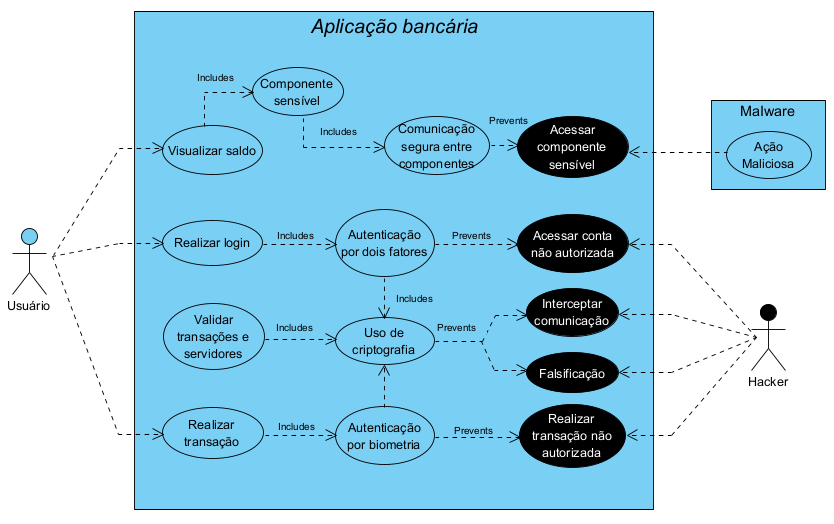
\includegraphics[width=17cm]{Imagens/misuse.png} 
    \caption{Casos de uso indevidos de aplicações bancárias}
    \label{misuses}
    \end{figure}
    
    Ao analisar essas ameaças, como malwares que visam roubo de credenciais e dados pessoais, fica clara a necessidade do desenvolvimento de requisitos que detalhem a implementação de mecanismos de segurança na comunicação entre processos na plataforma Android para proteção desses componentes sensíveis. 
    
    Similarmente, a identificação de vulnerabilidades em processos de autenticação deixa claro a importância da adoção de métodos de autenticação mais robustos, como autenticação multifator (MFA), biometria e pins numéricos, para mitigar riscos de acesso não autorizado.

    A criptografia, por sua vez, é fundamental para garantir a segurança dos dados em trânsito e em repouso. A análise dos casos de uso indevido encaminha a escolha de padrões criptográficos modernos que são capazes de resistir a ataques sofisticados, como AES-256-CBC, ECDSA e SHA-256. 
    
    Finalmente, a necessidade de proteger a comunicação entre o cliente e o servidor contra ataques de rede, como os ataques MITM, destaca diretamente a importância da adoção de protocolos de comunicação seguros, como o Transport Layer Security (TLS) 1.3.

    \section{Definição dos requisitos}
    Durante o processo de estudo, o objetivo foi encontrar um conjunto de pontos críticos e suas respectivas remediações de modo a entender as aplicações bancárias e por fim propor um modelo teórico capaz de tornar o ambiente seguro para o uso. A partir da análise do cenários de ameaças anterior, foi obtida uma base para a realização da definição dos requisitos de segurança necessários para mitigar esses riscos associados. Esses requisitos foram divididos em áreas como visto na figura \ref{visao}.

    \begin{figure}[H]
    \centering 
    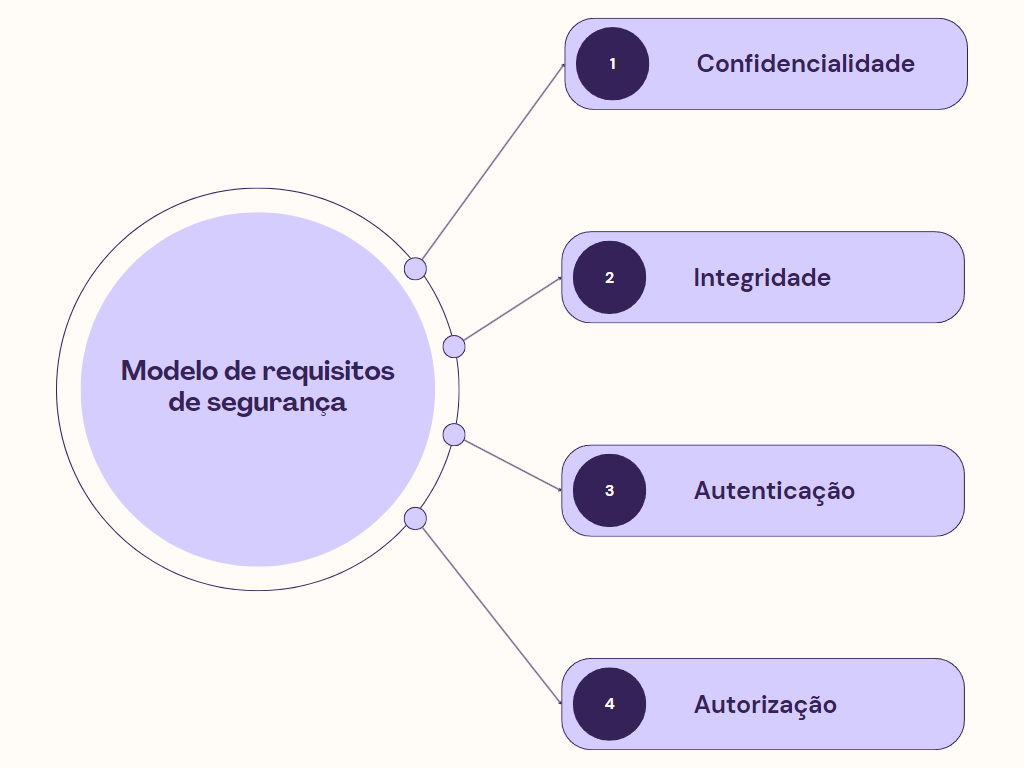
\includegraphics[width=10cm]{Imagens/arvre.png} 
    \caption{Visão geral dos requisitos de segurança}
    \label{visao}
    \end{figure}

    \begin{enumerate}

    \subsection{Requisitos de confidencialidade}

    \item O sistema deverá utilizar criptografia para armazenar senhas e chaves.
    
    \item A aplicação deverá utilizar TLS para realizar a comunicação com o servidor.
    
    \subsection{Requisitos de integridade}

    \item O sistema deverá armazenar o Hash de cada transação.

    \item O sistema deverá armazenar a assinatura digital do pagador em cada transação.

    \item O sistema deverá realizar a comunicação apenas com o servidor confiável.
    
    \subsection{Requisitos de autenticação}

    \item O acesso ao sistema deverá ser feito utilizando autenticação de multiplos fatores (MFA).

    \item O sistema deverá exigir Pin ou biometria para a realização de transações e pagamentos. 
    
    \subsection{Requisitos de autorização}

    \item O sistema não deve exportar componentes que não exigem interação externa. 

    \item O sistema deve exigir permissões para acessar os componentes exportados. 

    \item O sistema deve validar de intents recebidas nos componentes exportados. 

    \end{enumerate}


    \section{Especificação dos requisitos de segurança}
    A especificação dos requisitos de segurança é um processo crítico que envolve o definição clara, detalhada e estruturada dos requisitos de segurança definidos anteriormente. Na prática, ela atua como um guia detalhado para desenvolvedores, engenheiros de qualidade e outros stakeholders, assegurando que todos tenham uma compreensão comum do que deve ser construído e como o sistema deve operar. Ela serve como uma ponte entre a análise de requisitos, onde as necessidades dos usuários e as restrições do sistema são identificadas, e a fase de desenvolvimento, onde essas necessidades são implementadas.
    
    \begin{enumerate}
    
        \subsection{Requisitos de Confidencialidade}
    
        \item \textbf{O sistema deverá utilizar criptografia para armazenar senhas e chaves}
        \begin{enumerate}
            \item[1.1] Identificar os dados que requerem criptografia.
            \item[1.2] Configurar o sistema para usar o algoritmo de criptografia Advanced Encryption Standard com uma chave de 256 bits no modo Cipher Block Chaining (AES-256-CBC) para senhas e chaves.
            \item[1.3] Gerar e armazenar chaves criptográficas de forma segura utilizando o Android KeyStore.
            \item[1.4] Utilizar os algoritmos para criptografar as senhas e chaves.
            \item[1.5] Armazenar o conteúdo criptografado no banco de dados.
            \item[1.6] Encerrar a sessão de criptografia e liberar os recursos de criptografia.
        \end{enumerate}
        
        \item \textbf{O sistema deverá utilizar TLS para realizar a comunicação}
        \begin{enumerate}
            \item[2.1] Configurar o sistema para estabelecer conexões seguras utilizando TLS 1.2 ou superior.
            \item[2.2] Iniciar a comunicação entre cliente e servidor.
            \item[2.3] Setar os parâmetros criptográficos do TLS com o servidor.
            \item[2.4] Verificar a validade do certificado digital do servidor.
            \item[2.5] Estabelecer a conexão TLS após a validação do certificado.
            \item[2.6] Transmitir dados de forma segura utilizando o canal TLS.
            \item[2.7] Encerrar a conexão TLS após a conclusão da comunicação.
        \end{enumerate}
    
        \subsection{Requisitos de Integridade}
    
        \item \textbf{O sistema deverá armazenar o Hash de cada transação}
        \begin{enumerate}
            \item[3.1] Gerar um hash criptográfico para cada transação utilizando o algoritmo Secure Hash Algorithm com valor hash de 256 bits (SHA-256).
            \item[3.2] Associar o hash à transação correspondente.
            \item[3.3] Verificar o hash ao acessar ou modificar a transação.
            \item[3.4] Armazenar o hash de forma segura no banco de dados.
            \item[3.5] Auditar periodicamente os hashes armazenados para garantir integridade.
            \item[3.6] Validar a consistência do hash durante o processamento das transações.
            \item[3.7] Registrar o resultado da validação de hash para auditoria futura.
        \end{enumerate}
    
        \item \textbf{O sistema deverá armazenar a assinatura digital do pagador em cada transação}
        \begin{enumerate}
            \item[4.1] Capturar a assinatura digital do pagador, feita com o algoritmo Elliptic Curve Digital Signature Algorithm (ECDSA), no momento da transação.
            \item[4.2] Validar a assinatura digital para garantir sua autenticidade.
            \item[4.3] Associar a assinatura digital à transação correspondente.
            \item[4.4] Armazenar a assinatura digital de forma segura no banco de dados.
            \item[4.5] Verificar a assinatura digital antes de processar a transação.
            \item[4.6] Auditar as assinaturas digitais armazenadas regularmente.
            \item[4.7] Registrar o status de verificação da assinatura digital para referência futura.
        \end{enumerate}
    
        \item \textbf{O sistema deverá realizar a comunicação apenas com o servidor confiável}
        \begin{enumerate}
            \item[5.1] Armazenar no código fonte da aplicação o certificado digital dos servidores confiáveis.
            \item[5.2] Configurar o cliente para usar exclusivamente os certificados digitais armazenados para comunicação.
            \item[5.3] Validar esses certificados digitais ao estabelecer uma conexão com o servidor.
            \item[5.4] Rejeitar conexões com servidores que não utilizem um dos certificados armazenados.
            \item[5.5] Registrar tentativas de conexão não autorizadas para análise de segurança.
        \end{enumerate}
    
        \subsection{Requisitos de Autenticação}
    
        \item \textbf{O acesso ao sistema deverá ser feito utilizando autenticação de multiplos fatores (MFA)}
        \begin{enumerate}
            \item[6.1] Exibir a interface de login para o usuário.
            \item[6.2] Solicitar nome de usuário e senha.
            \item[6.3] Verificar usuário e senha cadastrada.
            \item[6.4] Enviar senha de uso único baseada em tempo ao número cadastrado por SMS.
            \item[6.5] Solicitar a senha de uso.
            \item[6.6] Verificar senha.
            \item[6.7] Liberar o acesso ao perfil de usuário  após a validação dos dois fatores bem-sucedida.
            \item[6.8] Permitir acesso às funcionalidades do sistema.
            \item[6.9] Finalizar processo.
        \end{enumerate}
    
        \item \textbf{O sistema deverá exigir Pin ou biometria para a realização de transações e pagamentos}
        \begin{enumerate}
            \item[7.1] Solicitar Pin ou autenticação biométrica ao iniciar uma transação.
            \item[7.2] Verificar o Pin ou a biometria fornecida pelo usuário.
            \item[7.3] Validar a autenticidade do usuário antes de processar a transação.
            \item[7.4] Processar a transação ou pagamento após a validação bem-sucedida.
            \item[7.5] Registrar as transações realizadas para auditoria e análise de segurança.
            \item[7.6] Encerrar o processo de transação após confirmação e notificar o usuário.
        \end{enumerate}
    
        \subsection{Requisitos de Autorização}
    
        \item \textbf{O sistema não deve exportar componentes que não têm interação externa}
        \begin{enumerate}
            \item[8.1] Identificar componentes que não necessitam de interação externa.
            \item[8.2] Definir como ``false'' a exportação desses componentes.
            \item[8.3] Verificar a configuração de componentes para garantir que não estão exportados indevidamente.
            \item[8.4] Monitorar o sistema para identificar tentativas de acesso a componentes não exportados.
            \item[8.5] Registrar qualquer tentativa de interação não autorizada para auditoria.
            \item[8.6] Encerrar processos que tentem acessar componentes não exportados.
        \end{enumerate}
    
        \item \textbf{O sistema deve exigir permissões para acessar os componentes exportados}
        \begin{enumerate}
            \item[9.1] Identificar os componentes exportados da aplicação.
            \item[9.2] Definir o parâmetro protectionLevel como ``signature'' nesses componentes.
            \item[9.3] Definir o parâmetro permission como ``READ\_PROVIDER'' nos provedores de conteúdo.
            \item[9.4] Monitorar o sistema para identificar tentativas de acesso não autorizadas a esses componentes.
            \item[9.5] Registrar qualquer tentativa de interação não autorizada para auditoria.
            \item[9.6] Encerrar processos que tentem acessar componentes sem autorização.
        \end{enumerate}
    
        \item \textbf{O sistema deve validar intents recebidas nos componentes exportados}
        \begin{enumerate}
            \item[10.1] Capturar intents recebidas nos componentes exportados.
            \item[10.2] Verificar a autenticidade e a origem das intents recebidas.
            \item[10.3] Validar os dados contidos nas intents antes de processá-las.
            \item[10.4] Processar a intent se for validada com sucesso.
            \item[10.5] Registrar todas as intents recebidas para auditoria e análise de segurança.
            \item[10.6] Monitorar o comportamento dos componentes exportados para detectar intents suspeitas.
            \item[10.7] Encerrar o processamento de intents inválidas ou não autorizadas.
        \end{enumerate}
    
    \end{enumerate}

    
    \section{Modelagem de dados e processos}
    A modelagem de dados e processos é uma fase essencial no desenvolvimento de sistemas, servindo como a base para a construção de soluções tecnológicas que sejam eficientes, escaláveis e alinhadas com os objetivos organizacionais. Este processo envolve a representação estruturada das informações que o sistema irá manipular (modelagem de dados) e a definição dos fluxos de trabalho e das atividades que o sistema deve executar (modelagem de processos).
    
    Dessa forma, exploraremos os princípios e técnicas de modelagem de dados e processos, demonstrando como os requisitos de segurança se relacionam com o sistema e suas funcionalidades.
    
    \subsection{Diagramas UML}

    O diagrama de classe, visto na figura \ref{cript} representa a classe Cliente e seus atributos e métodos. A classe possui os atributos senha, que é uma informação considerada sensível no processo de armazenamento. Este diagrama sugere que os dados sensíveis, no caso a senha, seja criptografado dentro de um sistema bancário.

    \begin{figure}[H]
    \centering 
    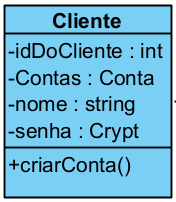
\includegraphics[width=6cm]{Imagens/cript.png} 
    \caption{Informações armazenadas em texto cifrado}
    \label{cript}
    \end{figure}

    O diagrama de sequência, observado na figura \ref{tls}, mostra o fluxo de interação entre a aplicação bancária e o servidor durante o processo da realização de uma comunicação criptografada, utilizando o TLS. A aplicação bancária envia uma lista de cifras com o conjunto de algoritmos que eles podem utilizar para a comunicação. Este conjunto tem vários parâmetros, sendo o primeiro o método de troca de chaves, o segundo o método de autenticação, terceiro o algoritmo simétrico com seu tamanho de chave e operação e por último o algoritmo de hash utilizado. Com isso, o servidor retorna a cifra escolhida, um certificado com uma assinatura digital e a server key exchange, que são os parâmetros utilizados para gerar a chave de criptografia. Dessa forma, a aplicação e o servidor conseguem realizar a comunicação criptografadas e segura.

    \begin{figure}[H]
    \centering 
    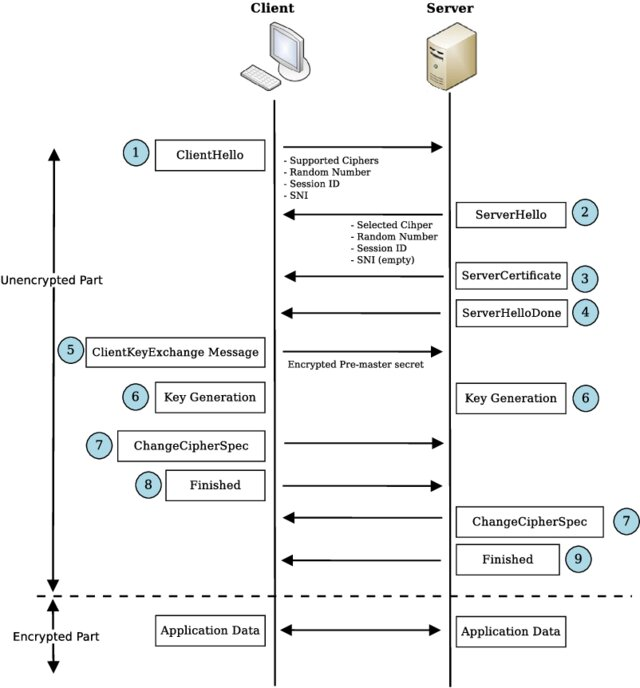
\includegraphics[width=13cm]{Imagens/tlshandshake.jpg} 
    \caption{Funcionamento do protocolo TLS}
    \label{tls}
    \cite{tls2016}
    \end{figure}

    O diagrama de classe, visto na figura \ref{transacao} representa a classe Transação e seus atributos e métodos. A classe possui os atributos verifIntegridade (responsável pela verificação de integridade de uma transação) e assinaturaDigital (Responsável pelo não repúdio e autenticidade da transação), utilizados para verificar a integridade e autenticidade dos dados. Este diagrama garante que os dados não foram alterados ou danificados dentro de um sistema bancário.
    
    \begin{figure}[H]
    \centering 
    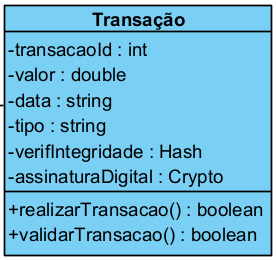
\includegraphics[width=6cm]{Imagens/integridade.png} 
    \caption{Armazenamento de Hash e Assinatura digital}
    \label{transacao}
    \end{figure}    

    O diagrama de sequência, observado na figura \ref{totp}, mostra o fluxo de interação entre um usuário, a aplicação bancária, o servidor e o banco de dados durante o processo de login. O usuário solicita o login e envia suas credenciais pré cadastradas. O servidor valida as credenciais consultando o banco de dados e, após a validação, solicita uma autenticação multifator (MFA). O usuário envia o MFA, que é validado, e uma sessão segura é gerada, resultando em um login bem-sucedido. 
    
    \begin{figure}[H]
    \centering 
    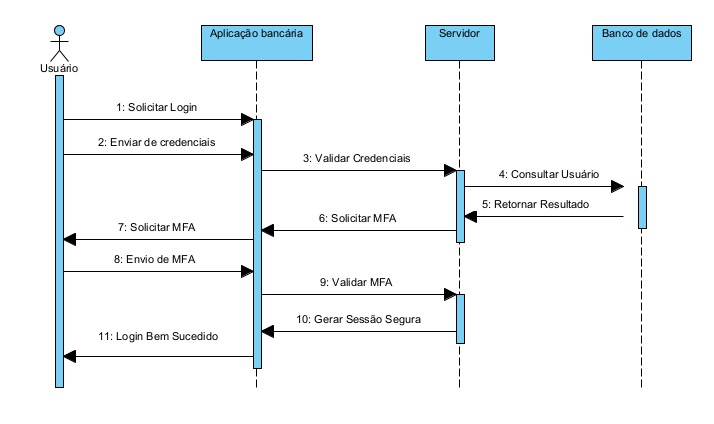
\includegraphics[width=15cm]{Imagens/login.png} 
    \caption{Autenticação multifatorial utilizando Login, Senha e TOTP}
    \label{totp}
    \end{figure}

    O diagrama de sequência, ilustrado na figura \ref{pin}, detalha o processo de solicitação e aprovação de uma transação ou pagamento. O usuário inicia a solicitação e envia um PIN para a aplicação bancária, que então o repassa ao servidor. O servidor valida os dados, verifica a integridade da transação e registra a operação no banco de dados. Após o registro, o servidor retorna o resultado, e a transação é aprovada. Este fluxo assegura que cada etapa seja validada e registrada adequadamente antes de concluir a transação.

    \begin{figure}[H]
    \centering 
    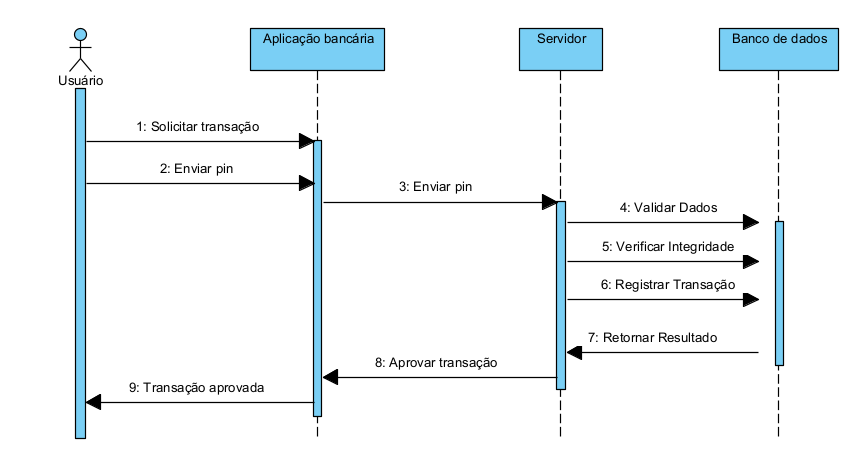
\includegraphics[width=15cm]{Imagens/pagamento.png} 
    \caption{Autenticação por Pin}
    \label{pin}
    \end{figure}

    O diagrama de caso de uso indevido, observado na figura \ref{malware}, ilustra a proteção de componentes sensíveis, exportados e consentidos em uma aplicação bancária contra ações maliciosas de malware. Para evitar ataques, são implementados controles como desabilitar a exportação de componentes (Exported:"false"), aplicar níveis de proteção (ProtectionLevel), e sanitarizar intents (IntentSanitizer). Esses mecanismos ajudam a mitigar as ações maliciosas que tentam explorar vulnerabilidades na aplicação.

    \begin{figure}[H]
    \centering 
    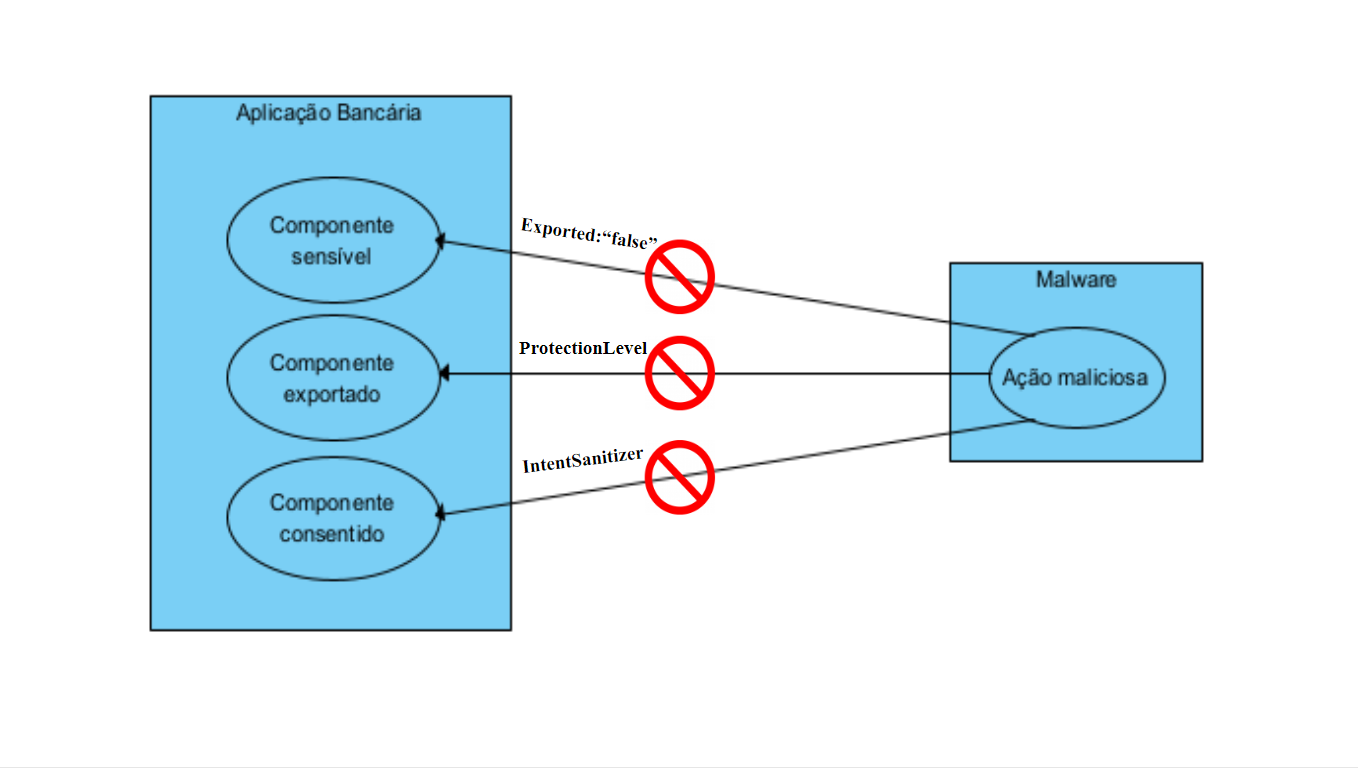
\includegraphics[width=14cm]{Imagens/malware.png} 
    \caption{Caso de uso indevido: ataque malware}
    \label{malware}
    \end{figure}
    

    \chapter{Estudo de caso e avaliação do modelo}
    Para validar o modelo de segurança proposto, utilizamos a aplicação ``Herd Financial'' do projeto GoatDroid para demonstração dos casos de uso dos requisitos de segurança modelados. Além disso, avaliamos a conformidade e garantia do modelo por meio da adequação à certificação de segurança PCI DSS.

    \section{Estudo de caso}
    Para avaliar a eficácia e viabilidade dos requisitos de segurança modelados por meio da demonstração dos casos de uso, adotamos uma abordagem estruturada dividida em duas etapas principais. Primeiro, identificamos e analisamos algumas das fragilidades presentes na aplicação Herd Financial, utilizando como referência o \citeonline{herd2016}, e logo após apontamos os requisitos de segurança modelados na etapa anterior capazes de mitigar essas vulnerabilidades, demonstrando exemplos de código em Java.


    \subsection{Visão Geral do Herd Financial}
    
    Herd Financial é uma aplicação bancária fictícia projetada pela \citeonline{goat2024} como parte do projeto GoatDroid, uma plataforma de teste para identificar e explorar vulnerabilidades em aplicações Android. O objetivo principal do Herd Financial é simular um ambiente de aplicação bancária real, permitindo que desenvolvedores e pesquisadores de segurança testem e compreendam as falhas comuns encontradas em aplicativos bancários móveis. A aplicação oferece funcionalidades típicas de um aplicativo bancário, como:

    \begin{itemize}[topsep=3pt, partopsep=3pt, itemsep=3pt, parsep=3pt]
        \item Visualização de Saldo: Os usuários podem verificar o saldo de suas contas bancárias.
        \item Transferência de Fundos: Permite a transferência de dinheiro entre contas.
        \item Gerenciamento de Contas: Inclui funcionalidades para adicionar, editar e remover contas bancárias.
        \item Histórico de Transações: Exibe um registro das transações realizadas pelo usuário.
    \end{itemize}

    Essas funcionalidades, enquanto fornecem um cenário realista para os usuários, também incorporam várias vulnerabilidades propositais. A presença dessas falhas intencionais faz do Herd Financial uma ferramenta valiosa para testar as práticas de segurança recomendadas e avaliar a eficácia das estratégias de mitigação.

    Através da análise do Herd Financial, podemos aplicar o modelo de segurança proposto e observar como ele se comporta em um ambiente de teste controlado. Isso nos permite identificar áreas de melhoria e validar a eficácia das medidas de segurança implementadas, oferecendo insights práticos que podem ser aplicados em desenvolvimentos futuros de aplicações bancárias reais.

    \subsection{Requisitos de autenticação e autorização}
    Herd Financial inicialmente utilizava um sistema básico de autenticação com senha mostrado na figura \ref{login}, sem suporte a autenticação multifatorial (MFA).

    \begin{figure}[H]
    \centering 
    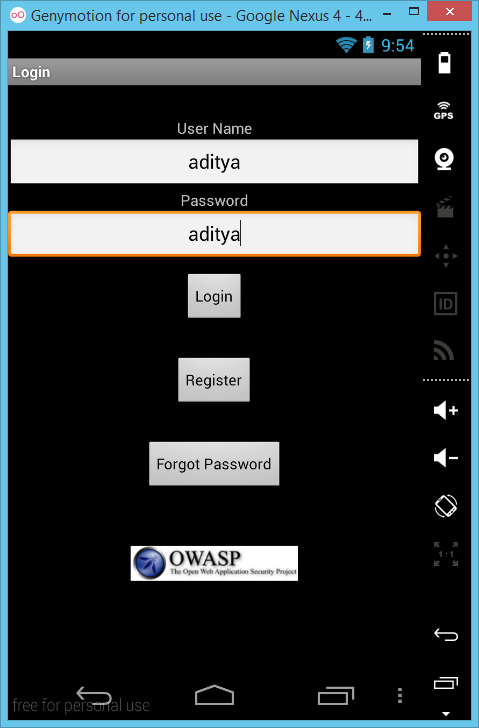
\includegraphics[width=7cm]{Imagens/loginherd.png} 
    \caption{Login de usuário do Herd Financial}
    Fonte: \citeonline{herd2016}
    \label{login}
    
    \end{figure}

    Este método simples de autenticação deixava a aplicação vulnerável a ataques de força bruta e acessos não autorizados. O modelo recomenda a autenticação multifatorial, adicionando uma camada adicional de segurança ao exigir um segundo fator de autenticação. No caso, um algoritmo TOTP.

    O código apresentado mostra como utilizar o Firebase para implementar o TOTP, onde um código temporário gerado por um aplicativo autenticador é requerido além da senha tradicional. Isso adiciona uma camada adicional de segurança, dificultando o acesso não autorizado mesmo que a senha do usuário seja comprometida.
    \\

    \begin{scriptsize}
    \estiloJava
    \begin{lstlisting}[caption={Autenticação por TOTP Utilizando Firebase}, label=lst:javacode]
    when (exception.resolver.hints[selectedIndex].factorId) {
        TotpMultiFactorGenerator.FACTOR_ID -> {
            val otpFromAuthenticator = // OTP escrito pelo usuário.
            val assertion = TotpMultiFactorGenerator.getAssertionForSignIn(
                exception.resolver.hints[selectedIndex].uid,
                otpFromAuthenticator
            )
            exception.resolver.resolveSignIn(assertion)
                .addOnSuccessListener { result ->
                    // Successfully signed in!
                    Log.d(TAG, "signInWithTOTP:success");
                }
                .addOnFailureListener { resolveError ->
                    Toast.makeText(TOTPActivity.this, "Invalid or expired OTP.",
                                Toast.LENGTH_SHORT).show();
                }
        }
    }
    \end{lstlisting}
    \end{scriptsize}

    Na maioria das vezes, após a autenticação em um aplicativo Android, o usuário é enviado para uma nova atividade com as funcionalidades da aplicação. Manter essas atividades exportadas e até mesmo sem permissões personalizadas, deixam a aplicação suscetível ao acesso não autorizado. 
    
    No aplicativo HerdFinancial, a atividade org.owasp.goatdroid.herdfinancial.activities.Main foi exportada e também não tem nenhuma permissão personalizada. O que permite a um malware simplesmente passar uma intenção e iniciar a atividade específica, como mostrado na figura \ref{drozer}.

    \begin{figure}[H]
    \centering 
    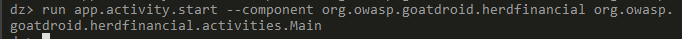
\includegraphics[width=16cm]{Imagens/drozer.png} 
    \caption{Acesso não autorizado utilizando Drozer}
    Fonte: \citeonline{herd2016}
    \label{drozer}
    \end{figure}

    Depois disso, o Herd Financial é iniciado com a conta padrão e podem ser feito coisas como transferir o dinheiro para a conta de outra pessoa, como vemos na figura \ref{main}. 

    \begin{figure}[H]
    \centering 
    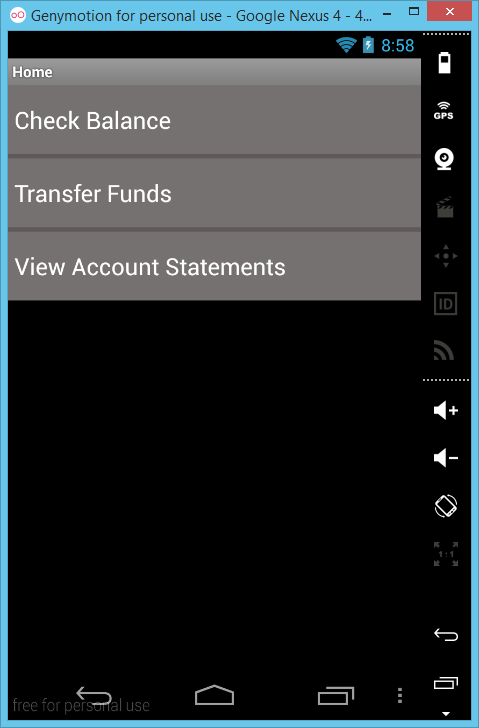
\includegraphics[width=6cm]{Imagens/acmain.png} 
    \caption{Tela inicial}
    Fonte: \citeonline{herd2016}
    \label{main}
    \end{figure}

    Ao utilizar as configurações corretas e permissões nos componente do android, bloqueamos esse tipo de interação. O modelo propõe uso de componentes exportados apenas quando necessário. 

    O código apresentado exemplifica como configurar componentes do Android para não serem exportados (android:exported="false"), garantindo que apenas o próprio aplicativo possa iniciar essas atividades. Ao limitar a exportação de componentes, o modelo previne que aplicativos externos interajam de forma indesejada com o aplicativo, aumentando a segurança contra acessos não autorizados.
    \\

    \begin{scriptsize}
    \estiloJava
    \begin{lstlisting}[caption={Componentes exportados}, label=lst:javacode]
    <activity android:name=".SensiveActivity" android:exported="false" >
        <intent-filter>
            <action android:name="EXAMPLE_ACTIVITY" />
            <category android:name="android.intent.category.LAUNCHER" />
        </intent-filter>
    </activity>

    <service
        android:name=".MessagingService"
        android:exported="false">
        <intent-filter>
            <action android:name="com.google.firebase.MESSAGING_EVENT" />
        </intent-filter>
    </service>

    <receiver android:name=".SensiveReceiver" android:exported="false">
        <intent-filter>
            <action android:name="EXAMPLE_BROADCAST" />
        </intent-filter>
    </receiver>
    
    \end{lstlisting}
    \end{scriptsize}


    Caso seja necessário a exportação, é fundamental definir permissões de segurança apropriadas e validar informações recebidas para componentes sensíveis. 

    O código demonstra como aplicar permissões de segurança apropriadas e filtrar intenções recebidas, garantindo que apenas aplicativos autorizados possam interagir com componentes sensíveis. Essa prática previne que dados sejam acessados ou manipulados por aplicativos não confiáveis, mitigando vulnerabilidades como ataques de malwares à aplicação.
    \\

    \begin{scriptsize}
    \estiloJava
    \begin{lstlisting}[caption={Permissões no Android e filtro de intenção}, label=lst:javacode]
    // Permissões
    <permission android:name="com.example.myapp.MY_PERMISSION" android:protectionLevel="signature" />
    
    <provider
        android:name=".MyContentProvider"
        android:authorities="com.example.myapp.provider"
        android:exported="true"
        android:permission="android.permission.READ_PROVIDER"
    </provider>


    // Verificação de intenção
    Intent intent = getIntent()
    Intent forward = (Intent) intent.getParcelableExtra("key");
    ComponentName name = forward.resolveActivity(getPackageManager());
    if (name.getPackageName().equals("safe_package") &&
            name.getClassName().equals("safe_class")) {
        startActivity(forward);
    }

    // Sanitização de intenção
    Intent intent = new  IntentSanitizer.Builder()
     .allowComponent("com.example.ActivityA")
     .allowData("com.example")
     .allowType("text/plain")
     .build()
     .sanitizeByThrowing(intent);
        
    \end{lstlisting}
    \end{scriptsize}

    Outra proteção recomendada para esses casos é o uso de Pin ou biometria para validar as ações do usuário. Assim garantindo que mesmo em contas comprometidas não seja possível realizar ações maliciosas.

    O código fornecido implementa autenticação biométrica em Android, garantindo que transações e pagamentos, só possam ser realizadas após a validação da identidade do usuário através de biometria. Isso adiciona uma camada extra de segurança, protegendo as ações do usuário contra acessos não autorizados, mesmo em casos onde a senha tenha sido comprometida.
    \\

    \begin{scriptsize}
    \estiloJava
    \begin{lstlisting}[caption={Autenticação por digital}, label=lst:javacode]
    private Executor executor;
    private BiometricPrompt biometricPrompt;
    private BiometricPrompt.PromptInfo promptInfo;
    
    @Override
    protected void onCreate(Bundle savedInstanceState) {
        super.onCreate(savedInstanceState);
        setContentView(R.layout.activity_login);
        executor = ContextCompat.getMainExecutor(this);
        biometricPrompt = new BiometricPrompt(MainActivity.this,
                executor, new BiometricPrompt.AuthenticationCallback() {
            @Override
            public void onAuthenticationError(int errorCode,
                    @NonNull CharSequence errString) {
                super.onAuthenticationError(errorCode, errString);
                Toast.makeText(getApplicationContext(),
                    "Authentication error: " + errString, Toast.LENGTH_SHORT)
                    .show();
            }
    
            @Override
            public void onAuthenticationSucceeded(
                    @NonNull BiometricPrompt.AuthenticationResult result) {
                super.onAuthenticationSucceeded(result);
                Toast.makeText(getApplicationContext(),
                    "Authentication succeeded!", Toast.LENGTH_SHORT).show();
            }
    
            @Override
            public void onAuthenticationFailed() {
                super.onAuthenticationFailed();
                Toast.makeText(getApplicationContext(), "Authentication failed",
                    Toast.LENGTH_SHORT)
                    .show();
            }
        });
    
        promptInfo = new BiometricPrompt.PromptInfo.Builder()
                .setTitle("Biometric login for my app")
                .setSubtitle("Log in using your biometric credential")
                .setNegativeButtonText("Use account password")
                .build();
    

        Button biometricLoginButton = findViewById(R.id.biometric_login);
        biometricLoginButton.setOnClickListener(view -> {
                biometricPrompt.authenticate(promptInfo);
        });
    }
    \end{lstlisting}
    \end{scriptsize}
    

    \subsection{Requisitos de confidencialidade e integridade}

    Outro ponto importante são as informações armazenadas pela aplicação. Como podemos ver na figura \ref{chave}, o Herd Financial armazena chaves sensíveis no código fonte do aplicativo. Dessa forma, qualquer um com o arquivo da aplicação pode obter a senha usando engenharia reversa.

    \begin{figure}[H]
    \centering 
    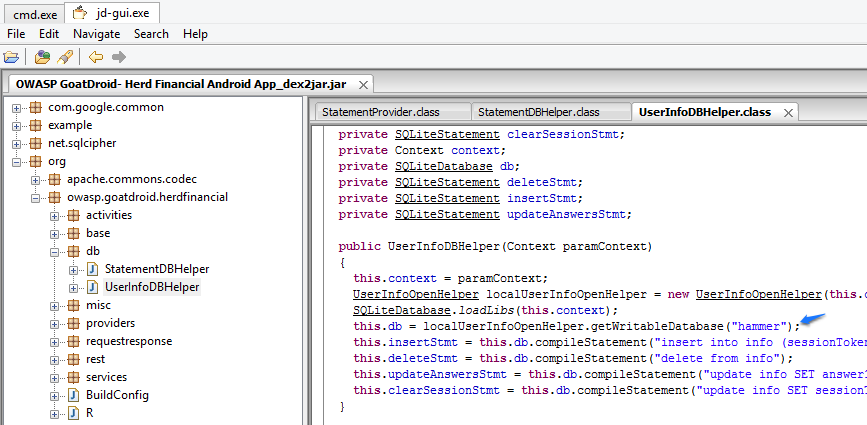
\includegraphics[width=14cm]{Imagens/hammer.png} 
    \caption{Informação vazada no código fonte}
    Fonte: \citeonline{herd2016}
    \label{chave}
    \end{figure}

    Além disso, a aplicação também guarda credenciais no armazenamento interno do dispositivo, como podemos ver nas imagens \ref{internal}, o que torna possível aos usuários maliciosos visualizar e utilizar essas informações. 
    
    \begin{figure}[H]
    \centering 
    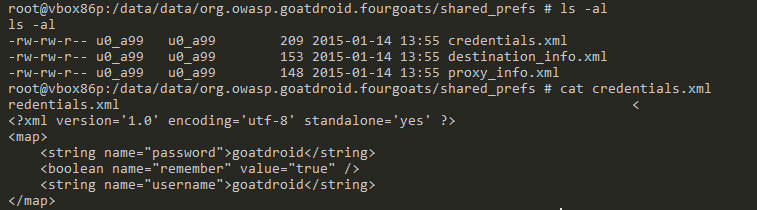
\includegraphics[width=15cm]{Imagens/internal.png} 
    \caption{Informação salva no armazenamento interno}
    Fonte: \citeonline{herd2016}
    \label{internal}
    \end{figure}


    Desse modo, o modelo proposto recomenda o uso de métodos de criptografia para o armazenamento de chaves e senhas. O uso de criptografia forte não só dificulta o acesso não autorizado, mas também garante a confidencialidade das informações, mesmo em caso de comprometimento de outros mecanismos de segurança.

    O código apresentado utiliza criptografia AES com chave de 256 bits e modo de operação CBC ou SHA-256 para proteger dados sensíveis armazenados localmente. A criptografia assegura que, mesmo se um atacante acessar o armazenamento, os dados permanecerão ininteligíveis sem a chave de decriptação correta, garantindo a confidencialidade das informações armazenadas.
    \\

    \begin{scriptsize}
    \estiloJava
    \begin{lstlisting}[caption={Uso de criptografia para armazenamento de dados}, label=lst:javacode]
    // Criptografia assimétrica utilizando o algoritmo AES
    byte[] plaintext = "Texto plano";
    KeyGenerator keygen = KeyGenerator.getInstance("AES");
    keygen.init(256);
    SecretKey key = keygen.generateKey();
    Cipher cipher = Cipher.getInstance("AES/CBC/PKCS5PADDING");
    cipher.init(Cipher.ENCRYPT_MODE, key);
    byte[] ciphertext = cipher.doFinal(plaintext);
    byte[] iv = cipher.getIV();


    // Criptografia de Hash utilizando o algoritmo SHA-256
    byte[] message = "Texto plano";
    MessageDigest md = MessageDigest.getInstance("SHA-256");
    byte[] digest = md.digest(message);
    
    \end{lstlisting}
    \end{scriptsize}

    Seguindo a mesma lógica, a aplicação também tem fragilidades encontradas nos dados em transito. O uso de métodos de criptografia fracos e a falta de verificações de certificados digitais permite que atacantes realizem ataques man-in-the-middle, interceptando e manipulando a comunicação entre o aplicativo e o servidor, como vemos na figura \ref{burp}. 

    \begin{figure}[H]
    \centering 
    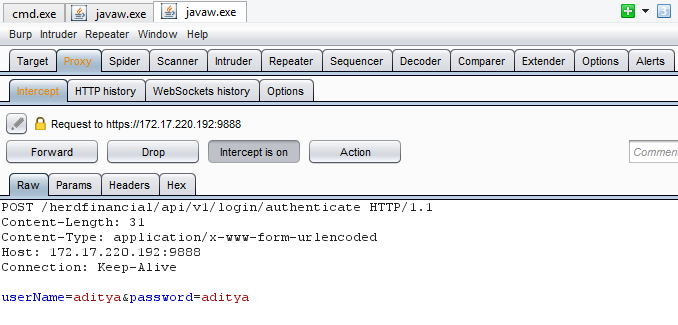
\includegraphics[width=14cm]{Imagens/burp.png} 
    \caption{Informação interceptada por proxy}
    Fonte: \citeonline{herd2016}
    \label{burp}
    \end{figure}

    O modelo proposto recomenda o uso do TLS para que as informações sejam transmitidas através de uma conexão que é totalmente criptografada e que a autenticidade tanto do servidor quanto do cliente sejam verificadas por meio de certificados digitais. 

    O código implementa uma conexão segura usando SSLSocket, que estabelece uma comunicação criptografada através de TLS. Isso garante que os dados transmitidos entre o cliente e o servidor sejam protegidos contra interceptação e manipulação, preservando a integridade e a confidencialidade das informações em trânsito.
    \\

    \begin{scriptsize}
    \estiloJava
    \begin{lstlisting}[caption={Conexão criptografada com SSLSocket}, label=lst:javacode]
    SSLSocketFactory socketFactory;
    SSLSocket socket;
    socketFactory = (SSLSocketFactory) SSLSocketFactory.getDefault();
    try {
        socket = (SSLSocket) socketFactory.createSocket(IP, Porta);
        System.out.println("Connected!");
    } catch (IOException e) {
        e.printStackTrace();
    }
    \end{lstlisting}
    \end{scriptsize}

    
    Por fim, nota-se que a aplicação não utiliza nenhuma forma de manter a integridade da mesma, o que permite a um atacante alterar transações ou até a própria aplicação. Dessa foram, o modelo recomenda a utilização de assinatura digital com algoritmos de criptografia assimétrica para garantir a procedência das informações e algoritmos de hash para garantir a integridade. 

    O código implementa uma assinatura digital usando o algoritmo ECDSA e verifica a integridade dos dados utilizando o hash criptográfico SHA-256. A assinatura digital garante que os dados ou transações não foram alterados desde que foram assinados, enquanto o hash criptográfico assegura que o conteúdo não foi modificado, protegendo assim a integridade e a autenticidade das informações.
    \\

    \begin{scriptsize}
    \estiloJava
    \begin{lstlisting}[caption={Assinatura digital com ECDSA e Hash criptográfico utilizando SHA-256}, label=lst:javacode]
    // Gerando uma assinatura digital
    byte[] message = "Texto plano";
    PrivateKey key = "Chave Privada";
    Signature s = Signature.getInstance("SHA256withECDSA");
    s.initSign(key);
    s.update(message);
    byte[] signature = s.sign();

    // Verificando uma assinatura digital
    byte[] message = "Texto plano";
    byte[] signature = "Assinatura";
    PublicKey key = "Chave Pública";
    Signature s = Signature.getInstance("SHA256withECDSA");
    s.initVerify(key);
    s.update(message);
    boolean valid = s.verify(signature);


    // Criptografia de Hash utilizando o algoritmo SHA-256
    byte[] message = "Texto plano";
    MessageDigest md = MessageDigest.getInstance("SHA-256");
    byte[] digest = md.digest(message);
    
    \end{lstlisting}
    \end{scriptsize}

    \section{Avaliação}

    A avaliação do modelo de segurança foi feita por meio da certificação PCI DSS, citada na seção \ref{pci} e desenvolvido pela \citeonline{pci2022}, com a verificação do cumprimento de 12 requisitos fundamentais exigidos pela organização. A conformidade com o PCI DSS não é apenas uma exigência das principais bandeiras de cartão de crédito, mas também uma medida crítica para minimizar riscos e fortalecer a confiança dos consumidores. Estes requisitos são projetados para cobrir todos os aspectos críticos da segurança da informação, desde a proteção da infraestrutura de rede até a implementação de políticas de segurança organizacional. 

    Na tabela \ref{tab:pci12} são mostrados os 12 requisitos exigidos pela certificação e marcados com ``X'' os quais o modelo proposto contempla. 

    \begin{table}[!htb]
    \centering
    \caption{12 requisitos do PCI DSS}
    \label{tab:pci12}
    \begin{tabular}{|l|c|}
    \hline
    \multicolumn{1}{|c|}{\textbf{Principais Requisitos do PCI DSS}}                                                                                                               & \textbf{Modelo} \\ \hline
    Instalar e manter controles de segurança de rede                                                                                                                     & X               \\ \hline
    \begin{tabular}[c]{@{}l@{}}Aplicar as configurações de segurança para todos os componentes de \\ sistema\end{tabular}                                                & X               \\ \hline
    Proteger os dados da conta armazenados                                                                                                                               & X               \\ \hline
    \begin{tabular}[c]{@{}l@{}}Proteger os dados do titular do cartão com criptografia forte durante\\ a transmissão em redes públicas abertas\end{tabular}              & X               \\ \hline
    Proteger todos os sistemas e redes de software malicioso                                                                                                             & X               \\ \hline
    Desenvolver e manter sistemas e software seguros                                                                                                                     & X               \\ \hline
    \begin{tabular}[c]{@{}l@{}}Restringir o acesso aos componentes de sistema e aos dados do titular\\ do cartão por necessidade de conhecimento do negócio\end{tabular} & X               \\ \hline
    Identificar usuários e autenticar o acesso aos componentes de sistema                                                                                                & X               \\ \hline
    Restringir o acesso físico aos dados do titular do cartão                                                                                                            &                 \\ \hline
    \begin{tabular}[c]{@{}l@{}}Registrar e monitorar todo o acesso aos componentes de sistema e \\ dados do titular do cartão\end{tabular}                               &                 \\ \hline
    Testar a segurança de sistemas e redes regularmente                                                                                                                  &                 \\ \hline
    Apoiar a segurança com políticas e programas organizacionais                                                                                           &                 \\ \hline
    \end{tabular}
    \end{table}

    \subsection{Análise de adequação}

    A seguir, é apresentada uma análise do modelo de requisitos de segurança para aplicações bancárias no Android em relação aos 12 requisitos fundamentais do PCI DSS, organizados em suas respectivas categorias. 

    \begin{enumerate}
        \item Construir e manter uma rede e sistemas seguros
            \begin{enumerate}
            \item \textbf{Instalar e manter controles de segurança de rede:} O modelo proposto não menciona explicitamente o uso de controles de monitoramento de rede, como firewalls ou IPS. Entretanto, ele restringe a interceptação de rede por meio do armazenamento dos certificados digitais confiáveis. 
            \item \textbf{Aplicar as configurações de segurança para todos os componentes de sistema:} O modelo sugere configurações de segurança para componentes do Android, como o uso de permissões rigorosas e validação de componentes, o que atende a este requisito.
            \end{enumerate}

        \item Proteger os dados da conta
            \begin{enumerate}
            \item \textbf{Proteger os dados da conta armazenados:} O modelo aborda a proteção dos dados armazenados com criptografia forte, como AES-256-CBC e SHA-256, o que cumpre este requisito.
            \item \textbf{Proteger os dados do titular do cartão com criptografia forte durante a transmissão em redes públicas abertas:} O uso de TLS 1.3 para criptografia de dados em trânsito, conforme recomendado no modelo, atende a este requisito.
            \end{enumerate}

        \item Manter um programa de gestão de vulnerabilidade
            \begin{enumerate}
            \item \textbf{Proteger todos os sistemas e redes de software malicioso:} O modelo menciona o uso de mecanismos de segurança da própria plataforma Android para proteção contra malwares, o que satisfaz este requisito. 
            \item \textbf{Desenvolver e manter sistemas e software seguros:} O modelo aborda a segurança durante o desenvolvimento de aplicações, o que é alinhado com este requisito. 
            \end{enumerate}

        \item Implementar medidas fortes de controle de acesso
            \begin{enumerate}
            \item \textbf{Restringir o acesso aos componentes de sistema e aos dados do titular do cartão por necessidade de conhecimento do negócio:} O modelo propõe a utilização de medidas de segurança nativas, como verificação e sanitização de intenções e uso de permissões, que são medidas adequadas para restringir o acesso com base na necessidade da plataforma; assim, contemplando este requisito. 
            \item \textbf{Identificar usuários e autenticar o acesso aos componentes de sistema:} A proposta de autenticação multifatorial (MFA) e autenticação de cada ação do usuário atende a este requisito.
            \item \textbf{Restringir o acesso físico aos dados do titular do cartão:} O modelo proposto  foca em controles de acesso digital e não aborda o controle de acesso físico. 
            \end{enumerate}

        \item Monitorar e testar as redes regularmente
            \begin{enumerate}
            \item \textbf{Registrar e monitorar todo o acesso aos componentes de sistema e dados do titular do cartão:} O modelo não contempla práticas de monitoramento e logging.
            \item \textbf{Testar a segurança de sistemas e redes regularmente:} O modelo não contempla recomendações de testes de segurança.
            \end{enumerate}

        \item Manter uma política de segurança da informação
            \begin{enumerate}
            \item \textbf{Apoiar a segurança da informação com políticas e programas organizacionais:} O modelo não menciona explicitamente a existência de políticas e programas organizacionais de segurança da informação.
            \end{enumerate}
    \end{enumerate}


    \subsection{Defesa do modelo}
    
    O modelo de segurança proposto cobre muitos dos aspectos fundamentais de segurança, como criptografia, autenticação, e controle de acesso, que são exigidos pelo PCI DSS. Em contraponto, algumas áreas, principalmente as relacionadas a infraestrutura e governança, não são contempladas, o que não garante conformidade total com a certificação PCI DSS. 

    Entretanto, como o resultado deste trabalho é um modelo de requisitos de segurança desenvolvido especificamente para aplicações bancárias no Android, a adequação do modelo ao seu propósito é demonstrada. O modelo foi elaborado para abordar os desafios únicos e as ameaças específicas enfrentadas por aplicações financeiras móveis, garantindo assim que as soluções propostas sejam diretamente aplicáveis e eficazes no contexto do Android.

    Portanto, afirmamos a adequação do modelo de requisitos de segurança proposto, pois ele fornece uma estrutura abrangente e direcionada para a proteção das aplicações bancárias no Android, considerando as necessidades específicas dessa plataforma e as expectativas do setor financeiro em termos de segurança e conformidade; chegando a conclusão que ele garante a segurança da informação.

    \section{Considerações finais do trabalho}
    O trabalho revelou diversas vulnerabilidades comuns em aplicações bancárias para Android, entre as principais ameaças identificadas estão os ataques de malware, falhas na autenticação, criptografia fraca e vulnerabilidades de rede. Os achados desta análise corroboram com o referencial teórico discutido anteriormente, especialmente com as diretrizes e recomendações da OWASP Mobile Top 10 descritas no tópico \ref{owasp} que engloba a maioria das ameaças citadas na literatura relacionada a segurança das aplicações bancárias. Dessa forma, fica evidente, tanto na literatura quanto nos resultados deste estudo, a importância dos requisitos de segurança bem definidos.

    Também nota-se que o resultado obtido neste estudo, isso é, o modelo de requisitos de segurança; está em consonância com as melhores práticas e recomendações encontradas na literatura sobre segurança em aplicações móveis, especialmente no contexto bancário. Os resultados deste estudo não apenas confirmam as melhores práticas recomendadas pelos artigos citados, encontrados na seção \ref{bancos}, mas também proporcionam uma definição, modelagem e avaliação de requisitos de segurança no cenário específico. 

    Com isso, a contribuição central deste estudo está na integração e na modelagem das práticas recomendadas encontradas na literatura em um modelo de segurança que destaca a relevância e a importância das medidas de segurança implementadas. Ao integrar e modelar informações de diversos artigos, conseguimos desenvolver um conjunto de práticas que pode servir como referência para a criação de futuras aplicações bancárias móveis seguras. O estudo de caso dos requisitos de segurança propostos mostrou-se eficaz na mitigação de vulnerabilidades, aprimorando significativamente a segurança da aplicação. O estudo de caso evidenciou como os requisitos de segurança modelados se comportam no cenário financeiro, demonstrando a importância de práticas de segurança bem estruturadas e contínuas para proteger aplicações bancárias móveis.

    Dessa forma, o modelo proposto nessa monografia têm implicações práticas significativas para desenvolvedores de aplicativos bancários, instituições financeiras e especialistas em cibersegurança. A implementação desses requisitos de segurança podem gerar sérios impactos positivos no desenvolvimento de aplicações bancárias no Android. Dentre elas o aumento da segurança das aplicações e da confiança dos clientes, com a implementação de medidas de segurança avançadas; a redução de riscos e custos, com a proteção da reputação da instituição financeira associado a diminuição dos riscos, violações de segurança e ataques cibernéticos; e melhores adaptações à regulamentações de segurança, com o auxílio para instituições financeiras a estar em conformidade com regulamentações rigorosas de proteção de dados. 
    
    Apesar dos resultados promissores esperados com a implementação do modelo de segurança para aplicações bancárias no Android, este estudo apresenta algumas limitações que devem ser consideradas. Primeiramente, a validação das medidas de segurança foi realizada em um ambiente controlado e teórico. Embora esse ambiente tenha permitido a avaliação detalhada de cada componente do modelo, ele não reproduz completamente as condições e desafios encontrados em ambientes de produção reais e práticos, onde fatores como a diversidade de dispositivos, versões do sistema operacional e comportamentos de usuários podem influenciar a eficácia das medidas de segurança implementadas.
    
    Além disso, a natureza dinâmica das ameaças à segurança cibernética implica que novas vulnerabilidades e métodos de ataque podem surgir continuamente. O modelo proposto, embora robusto, pode necessitar de atualizações e adaptações constantes para se manter eficaz contra novas formas de ataque. A rapidez com que essas ameaças evoluem pode superar a capacidade do modelo de responder em tempo hábil, especialmente se não houver um processo de monitoramento e atualização contínuo. Com isso, a sofisticação crescente dos ataques requer uma colaboração entre a indústria e a academia a fim de encontrar soluções inovadoras e uma abordagem proativa à segurança.

    Outro ponto a ser destacado é a especificação relacionada ao escopo das funcionalidades avaliadas. Este estudo focou principalmente em medidas de segurança diretamente relacionada as entendidas maiores ameaças encontradas em aplicações bancárias. No entanto, devem ser avaliadas todas as ameaças catalogadas e outras áreas da segurança também devem ser levadas em consideração durante a implementação de qualquer aplicação bancárias.

    \chapter{Conclusão}
    
    Esta monografia teve como objetivo desenvolver um modelo de requisitos de segurança robusto para aplicações bancárias no Android, utilizando como base os principais desafios, ameaças, melhores práticas e recomendações para mitigação encontradas na literatura. Verificou-se que garantir a segurança em aplicativos bancários móveis é uma área complexa que exige uma abordagem multifacetada para proteger os dados do usuário e manter a integridade das transações financeiras.

    Durante a pesquisa, várias dificuldades foram encontradas, impactando o desenvolvimento do trabalho, especialmente em relação à obtenção, filtragem e análise de informações. A rápida evolução das ameaças e das tecnologias de segurança em aplicações bancárias móveis tornou desafiador manter uma revisão bibliográfica atualizada. Além disso, a grande quantidade de estudos listados com as palavras chaves pesquisadas dificultou a filtragem de informações relevantes e a identificação de padrões consolidados e práticas recomendadas. Essas dificuldades exigiram uma abordagem meticulosa e adaptável na análise das informações disponíveis, além de um esforço adicional na busca por fontes alternativas e confiáveis para fundamentar o trabalho.

    O principal resultado desta pesquisa é o modelo de requisitos de segurança fornecido para fomentar a segurança da informação dos aplicativos bancários Android.

    Primeiramente, a fase de elicitação de requisitos permitiu uma compreensão aprofundada das ameaças e vulnerabilidades específicas associadas a aplicações bancárias móveis. Através da análise da literatura e do estudo de casos de uso indevido, foram identificados os principais pontos críticos que precisavam ser abordados e utilizados ao definir, especificar e modelar os requisitos de segurança. Esta etapa foi essencial para garantir que o modelo de segurança desenvolvido fosse alinhado com as necessidades reais e práticas do setor bancário. 
    
    Essas contribuições estabeleceram um modelo de segurança abrangente, focado nos pilares da confidencialidade, integridade, autenticação e autorização. O modelo desenvolvido assegura que todas as comunicações e dados dentro da aplicação bancária sejam protegidos contra acessos não autorizados, garantindo que apenas entidades legítimas possam acessar informações sensíveis. A integridade é mantida através de verificações rigorosas e mecanismos de validação, prevenindo alterações não autorizadas nos dados. A autenticação robusta e a autorização rigorosa garantem que somente usuários e processos devidamente verificados possam realizar ações críticas na aplicação. 

    Por fim, a avaliação do modelo de requisitos de segurança foi realizada através de um estudo de caso aplicado à aplicação bancária Herd Financial e por um estudo de adequação a certificação de segurança financeira PCI DSS. Estes estudos envolveram a implementação teórica dos requisitos propostos a fim de avaliar a viabilidade e aplicabilidade do modelo proposto e a sua adequação a certificação financeira renomada para avaliar sua eficácia e robustez. Dessa forma, oferecendo um caminho claro para desenvolvedores que buscam fortalecer a segurança de suas aplicações bancárias no Android.
    
    Assim, o trabalho proporciona uma base sólida e confiável, crucial para o desenvolvimento de aplicações bancárias móveis seguras no Android, abordando as necessidades fundamentais de segurança no cenário de ameaças cibernéticas em constante evolução.

    Entretanto, a sofisticação crescente dos ataques requer uma colaboração entre a indústria e a academia a fim de encontrar soluções inovadoras e uma abordagem proativa à segurança. Uma direção futura para o tema é a combinação de outras tecnologias à segurança da informação, como a inteligência artificial citada por  \citeonline{Oguntimilehin2022}, o IOT citado por \citeonline{Krishna2021}, e a implementação de novas formas de autenticação como dito por \citeonline{Hussein2022}; e como elas podem fornecer uma defesa eficaz contra essas ameaças.

% ----------------------------------------------------------
% Refer\^{e}ncias bibliogr\'{a}ficas
% ----------------------------------------------------------

\bibliography{Projeto,ZehluTCC}    %% arquivos *.bib
                                         %% FulanoTCCbib.bib \'{e} o arquvi exclusivo do TCC



\end{document}
